% This is samplepaper.tex, a sample chapter demonstrating the
%DIF LATEXDIFF DIFFERENCE FILE
%DIF DEL diffbase.tex                     Sun Apr 11 11:23:04 2021
%DIF ADD policar2020-tsne-embedding.tex   Mon Apr 12 12:46:43 2021
% LLNCS macro package for Springer Computer Science proceedings;
% Version 2.20 of 2017/10/04
%
\documentclass[runningheads]{llncs}
%
\usepackage{graphicx}
\usepackage{amsmath, amssymb}
\usepackage{multirow}
\usepackage{booktabs}
%DIF 11c11
%DIF < \usepackage{todo}
%DIF -------
\usepackage{hyperref} %DIF > 
%DIF -------

% Fixup hyphenation
\hyphenation{cor-res-pon-ding}
\hyphenation{cor-re-lat-tion}
\hyphenation{compa-rison}
\hyphenation{compa-risons}
\hyphenation{ini-tial-iza-tion}
\hyphenation{in-clud-ing}

\newcommand{\etal}{\textit{et al.}}
\newcommand{\beginsupplement}{% %DIF > 
  \setcounter{table}{0} %DIF > 
  \renewcommand{\thetable}{S\arabic{table}}% %DIF > 
  \setcounter{figure}{0} %DIF > 
  \renewcommand{\thefigure}{S\arabic{figure}}% %DIF > 
} %DIF > 
%DIF PREAMBLE EXTENSION ADDED BY LATEXDIFF
%DIF UNDERLINE PREAMBLE %DIF PREAMBLE
\RequirePackage[normalem]{ulem} %DIF PREAMBLE
\RequirePackage{color}\definecolor{RED}{rgb}{1,0,0}\definecolor{BLUE}{rgb}{0,0,1} %DIF PREAMBLE
\providecommand{\DIFaddtex}[1]{{\protect\color{blue}\uwave{#1}}} %DIF PREAMBLE
\providecommand{\DIFdeltex}[1]{{\protect\color{red}\sout{#1}}}                      %DIF PREAMBLE
%DIF SAFE PREAMBLE %DIF PREAMBLE
\providecommand{\DIFaddbegin}{} %DIF PREAMBLE
\providecommand{\DIFaddend}{} %DIF PREAMBLE
\providecommand{\DIFdelbegin}{} %DIF PREAMBLE
\providecommand{\DIFdelend}{} %DIF PREAMBLE
\providecommand{\DIFmodbegin}{} %DIF PREAMBLE
\providecommand{\DIFmodend}{} %DIF PREAMBLE
%DIF FLOATSAFE PREAMBLE %DIF PREAMBLE
\providecommand{\DIFaddFL}[1]{\DIFadd{#1}} %DIF PREAMBLE
\providecommand{\DIFdelFL}[1]{\DIFdel{#1}} %DIF PREAMBLE
\providecommand{\DIFaddbeginFL}{} %DIF PREAMBLE
\providecommand{\DIFaddendFL}{} %DIF PREAMBLE
\providecommand{\DIFdelbeginFL}{} %DIF PREAMBLE
\providecommand{\DIFdelendFL}{} %DIF PREAMBLE
%DIF HYPERREF PREAMBLE %DIF PREAMBLE
\providecommand{\DIFadd}[1]{\texorpdfstring{\DIFaddtex{#1}}{#1}} %DIF PREAMBLE
\providecommand{\DIFdel}[1]{\texorpdfstring{\DIFdeltex{#1}}{}} %DIF PREAMBLE
\newcommand{\DIFscaledelfig}{0.5}
%DIF HIGHLIGHTGRAPHICS PREAMBLE %DIF PREAMBLE
\RequirePackage{settobox} %DIF PREAMBLE
\RequirePackage{letltxmacro} %DIF PREAMBLE
\newsavebox{\DIFdelgraphicsbox} %DIF PREAMBLE
\newlength{\DIFdelgraphicswidth} %DIF PREAMBLE
\newlength{\DIFdelgraphicsheight} %DIF PREAMBLE
% store original definition of \includegraphics %DIF PREAMBLE
\LetLtxMacro{\DIFOincludegraphics}{\includegraphics} %DIF PREAMBLE
\newcommand{\DIFaddincludegraphics}[2][]{{\color{blue}\fbox{\DIFOincludegraphics[#1]{#2}}}} %DIF PREAMBLE
\newcommand{\DIFdelincludegraphics}[2][]{% %DIF PREAMBLE
\sbox{\DIFdelgraphicsbox}{\DIFOincludegraphics[#1]{#2}}% %DIF PREAMBLE
\settoboxwidth{\DIFdelgraphicswidth}{\DIFdelgraphicsbox} %DIF PREAMBLE
\settoboxtotalheight{\DIFdelgraphicsheight}{\DIFdelgraphicsbox} %DIF PREAMBLE
\scalebox{\DIFscaledelfig}{% %DIF PREAMBLE
\parbox[b]{\DIFdelgraphicswidth}{\usebox{\DIFdelgraphicsbox}\\[-\baselineskip] \rule{\DIFdelgraphicswidth}{0em}}\llap{\resizebox{\DIFdelgraphicswidth}{\DIFdelgraphicsheight}{% %DIF PREAMBLE
\setlength{\unitlength}{\DIFdelgraphicswidth}% %DIF PREAMBLE
\begin{picture}(1,1)% %DIF PREAMBLE
\thicklines\linethickness{2pt} %DIF PREAMBLE
{\color[rgb]{1,0,0}\put(0,0){\framebox(1,1){}}}% %DIF PREAMBLE
{\color[rgb]{1,0,0}\put(0,0){\line( 1,1){1}}}% %DIF PREAMBLE
{\color[rgb]{1,0,0}\put(0,1){\line(1,-1){1}}}% %DIF PREAMBLE
\end{picture}% %DIF PREAMBLE
}\hspace*{3pt}}} %DIF PREAMBLE
} %DIF PREAMBLE
\LetLtxMacro{\DIFOaddbegin}{\DIFaddbegin} %DIF PREAMBLE
\LetLtxMacro{\DIFOaddend}{\DIFaddend} %DIF PREAMBLE
\LetLtxMacro{\DIFOdelbegin}{\DIFdelbegin} %DIF PREAMBLE
\LetLtxMacro{\DIFOdelend}{\DIFdelend} %DIF PREAMBLE
\DeclareRobustCommand{\DIFaddbegin}{\DIFOaddbegin \let\includegraphics\DIFaddincludegraphics} %DIF PREAMBLE
\DeclareRobustCommand{\DIFaddend}{\DIFOaddend \let\includegraphics\DIFOincludegraphics} %DIF PREAMBLE
\DeclareRobustCommand{\DIFdelbegin}{\DIFOdelbegin \let\includegraphics\DIFdelincludegraphics} %DIF PREAMBLE
\DeclareRobustCommand{\DIFdelend}{\DIFOaddend \let\includegraphics\DIFOincludegraphics} %DIF PREAMBLE
\LetLtxMacro{\DIFOaddbeginFL}{\DIFaddbeginFL} %DIF PREAMBLE
\LetLtxMacro{\DIFOaddendFL}{\DIFaddendFL} %DIF PREAMBLE
\LetLtxMacro{\DIFOdelbeginFL}{\DIFdelbeginFL} %DIF PREAMBLE
\LetLtxMacro{\DIFOdelendFL}{\DIFdelendFL} %DIF PREAMBLE
\DeclareRobustCommand{\DIFaddbeginFL}{\DIFOaddbeginFL \let\includegraphics\DIFaddincludegraphics} %DIF PREAMBLE
\DeclareRobustCommand{\DIFaddendFL}{\DIFOaddendFL \let\includegraphics\DIFOincludegraphics} %DIF PREAMBLE
\DeclareRobustCommand{\DIFdelbeginFL}{\DIFOdelbeginFL \let\includegraphics\DIFdelincludegraphics} %DIF PREAMBLE
\DeclareRobustCommand{\DIFdelendFL}{\DIFOaddendFL \let\includegraphics\DIFOincludegraphics} %DIF PREAMBLE
%DIF LISTINGS PREAMBLE %DIF PREAMBLE
\RequirePackage{listings} %DIF PREAMBLE
\RequirePackage{color} %DIF PREAMBLE
\lstdefinelanguage{DIFcode}{ %DIF PREAMBLE
%DIF DIFCODE_UNDERLINE %DIF PREAMBLE
  moredelim=[il][\color{red}\sout]{\%DIF\ <\ }, %DIF PREAMBLE
  moredelim=[il][\color{blue}\uwave]{\%DIF\ >\ } %DIF PREAMBLE
} %DIF PREAMBLE
\lstdefinestyle{DIFverbatimstyle}{ %DIF PREAMBLE
	language=DIFcode, %DIF PREAMBLE
	basicstyle=\ttfamily, %DIF PREAMBLE
	columns=fullflexible, %DIF PREAMBLE
	keepspaces=true %DIF PREAMBLE
} %DIF PREAMBLE
\lstnewenvironment{DIFverbatim}{\lstset{style=DIFverbatimstyle}}{} %DIF PREAMBLE
\lstnewenvironment{DIFverbatim*}{\lstset{style=DIFverbatimstyle,showspaces=true}}{} %DIF PREAMBLE
%DIF END PREAMBLE EXTENSION ADDED BY LATEXDIFF

\begin{document}
%
\title{Embedding to Reference t-SNE Space Addresses Batch Effects in Single-Cell Classification}
%
\titlerunning{t-SNE Embedding and Batch Effects}
%
\author{Pavlin G. Poli\v{c}ar\inst{1} \and
Martin Stra\v{z}ar\inst{1} \and
Bla\v{z} Zupan\inst{1,2}}
%
\authorrunning{P. G. Poli\v{c}ar, M. Stra\v{z}ar, and B. Zupan}
%
\institute{University of Ljubljana, Faculty of Computer and Information Science, Večna pot 113, Ljubljana
\email{\{pavlin.policar,martin.strazar,blaz.zupan\}@fri.uni-lj.si}\\[2pt]
\and
Baylor College of Medicine, Houston, TX 77030, USA
}

\maketitle

\begin{abstract}

Dimensionality reduction techniques, such as t-SNE, can construct informative
visualizations of high-dimensional data. When jointly visualising multiple data
sets, a straightforward application of these methods often fails; instead of
revealing underlying classes, the resulting visualizations expose
dataset-specific clusters. To circumvent these batch effects, we propose an
embedding procedure that uses a t-SNE visualization constructed on a reference
data set as a scaffold for embedding new data points. Each data instance \DIFdelbegin \DIFdel{in the }\DIFdelend \DIFaddbegin \DIFadd{from a
new, unseen, }\DIFaddend secondary data is embedded independently and does not change the
reference embedding. This prevents any interactions between instances in the
secondary data and implicitly mitigates batch effects. We demonstrate the
utility of this approach by analyzing six recently published single-cell gene
expression data sets with up to tens of thousands of cells and thousands of
genes. The batch effects in our studies are particularly strong as the data
comes from different institutions using different experimental protocols. The
visualizations constructed by our proposed approach are clear of batch effects,
and the cells from secondary data sets correctly co-cluster with cells of the
same type from the primary data. We also show the predictive power of our
\DIFaddbegin \DIFadd{simple, }\DIFaddend visual classification approach in t-SNE space matches the accuracy of
\DIFaddbegin \DIFadd{specialized }\DIFaddend machine learning techniques that consider the entire compendium of
features that profile single cells.

\keywords{Batch Effects \and Embedding \and t-SNE \and Visualization \and Single-Cell Transcriptomics \and Data Integration \and Domain Adaptation.}
\end{abstract}


\section{Introduction}
\label{sec:intro}

Two-dimensional embeddings and their visualizations may assist in the analysis
and interpretation of high-dimensional data. Intuitively, two data instances
should be co-located in the resulting visualization if their multi-dimensional
profiles are similar. For this task, non-linear embedding techniques such as
t\nobreakdash -distributed stochastic neighbor embedding (t-SNE)~\DIFdelbegin \DIFdel{\mbox{%DIFAUXCMD
\cite{tsne} }\hspace{0pt}%DIFAUXCMD
}\DIFdelend \DIFaddbegin \DIFadd{\mbox{%DIFAUXCMD
\cite{Maaten2008} }\hspace{0pt}%DIFAUXCMD
}\DIFaddend or
uniform manifold approximation and projection~\DIFdelbegin \DIFdel{\mbox{%DIFAUXCMD
\cite{umap} }\hspace{0pt}%DIFAUXCMD
}\DIFdelend \DIFaddbegin \DIFadd{\mbox{%DIFAUXCMD
\cite{McInnes2018} }\hspace{0pt}%DIFAUXCMD
}\DIFaddend have recently
complemented traditional data transformation and embedding approaches such as
principal component analysis (PCA)\DIFaddbegin \DIFadd{~\mbox{%DIFAUXCMD
\cite{wold1987principal} }\hspace{0pt}%DIFAUXCMD
}\DIFaddend and multi-dimensional
scaling~\DIFdelbegin \DIFdel{\mbox{%DIFAUXCMD
\cite{distill,umap_single_cell}}\hspace{0pt}%DIFAUXCMD
}\DIFdelend \DIFaddbegin \DIFadd{\mbox{%DIFAUXCMD
\cite{cox2008multidimensional}}\hspace{0pt}%DIFAUXCMD
}\DIFaddend . While useful for visualizing data from
a single coherent source, these methods may encounter problems with multiple
data sources. Here, when performing dimensionality reduction on a merged data
set, the resulting visualizations would typically reveal source-specific
clusters instead of grouping data instances of the same class, regardless of
data sources. This source-specific confounding is often referred to as {\em
domain shift}~\cite{domain_shift}, {\em covariate shift}~\cite{covariate_shift}
or {\em data set shift}~\cite{dataset_shift}. In bioinformatics, the
domain-specific differences are more commonly referred to as {\em batch
effects}~\DIFdelbegin \DIFdel{\mbox{%DIFAUXCMD
\cite{cca,mnn,seurat}}\hspace{0pt}%DIFAUXCMD
}\DIFdelend \DIFaddbegin \DIFadd{\mbox{%DIFAUXCMD
\cite{Butler2018,Haghverdi2018,Stuart2019}}\hspace{0pt}%DIFAUXCMD
}\DIFaddend .

Massive, multi-variate biological data sets often suffer from these
source-specific biases.  The focus of this work is single-cell genomics, a
domain that was selected due to high biomedical relevance and abundance of
recently published data. Single-cell RNA sequencing (scRNA-seq) data sets are
the result of isolating RNA molecules from individual cells, which serve as an
estimate of the expression of cell's genes.  The studies can exceed thousands
of cells and tens of thousands of genes, and typically start with cell type
analysis. Here, it is expected that cells of the same type would cluster
together in two-dimensional data visualization~\DIFdelbegin \DIFdel{\mbox{%DIFAUXCMD
\cite{seurat}}\hspace{0pt}%DIFAUXCMD
}\DIFdelend \DIFaddbegin \DIFadd{\mbox{%DIFAUXCMD
\cite{Wolf2018}}\hspace{0pt}%DIFAUXCMD
}\DIFaddend . For instance,
Fig.~\ref{fig:batch_effect}.a shows t-SNE embedded data from mouse brain cells
originating from the visual cortex~\DIFdelbegin \DIFdel{\mbox{%DIFAUXCMD
\cite{hrvatin2018} }\hspace{0pt}%DIFAUXCMD
}\DIFdelend \DIFaddbegin \DIFadd{\mbox{%DIFAUXCMD
\cite{Hrvatin2018} }\hspace{0pt}%DIFAUXCMD
}\DIFaddend and the
hypothalamus~\DIFdelbegin \DIFdel{\mbox{%DIFAUXCMD
\cite{chen2017}}\hspace{0pt}%DIFAUXCMD
}\DIFdelend \DIFaddbegin \DIFadd{\mbox{%DIFAUXCMD
\cite{Chen2017}}\hspace{0pt}%DIFAUXCMD
}\DIFaddend . The figure reveals distinct clusters but also
separates the data from the two brain regions. These two regions share the same
cell types and --- contrary to the depiction in Fig.~\ref{fig:batch_effect}.a
--- we would expect the data points from the two studies to overlap. Batch
effects similarly prohibit the utility of t-SNE in the exploration of
pancreatic cells in Fig.~\ref{fig:batch_effect}.b, which renders the data from
a pancreatic cell atlas~\DIFdelbegin \DIFdel{\mbox{%DIFAUXCMD
\cite{baron2016} }\hspace{0pt}%DIFAUXCMD
}\DIFdelend \DIFaddbegin \DIFadd{\mbox{%DIFAUXCMD
\cite{Baron2016} }\hspace{0pt}%DIFAUXCMD
}\DIFaddend and similarly-typed cells from
diabetic patients~\DIFdelbegin \DIFdel{\mbox{%DIFAUXCMD
\cite{xin2016}}\hspace{0pt}%DIFAUXCMD
}\DIFdelend \DIFaddbegin \DIFadd{\mbox{%DIFAUXCMD
\cite{Xin2016}}\hspace{0pt}%DIFAUXCMD
}\DIFaddend . Just like with data from brain cells,
pancreatic cells cluster primarily by data source, again resulting in a
visualization driven by batch effects.

\begin{figure}[htbp]
  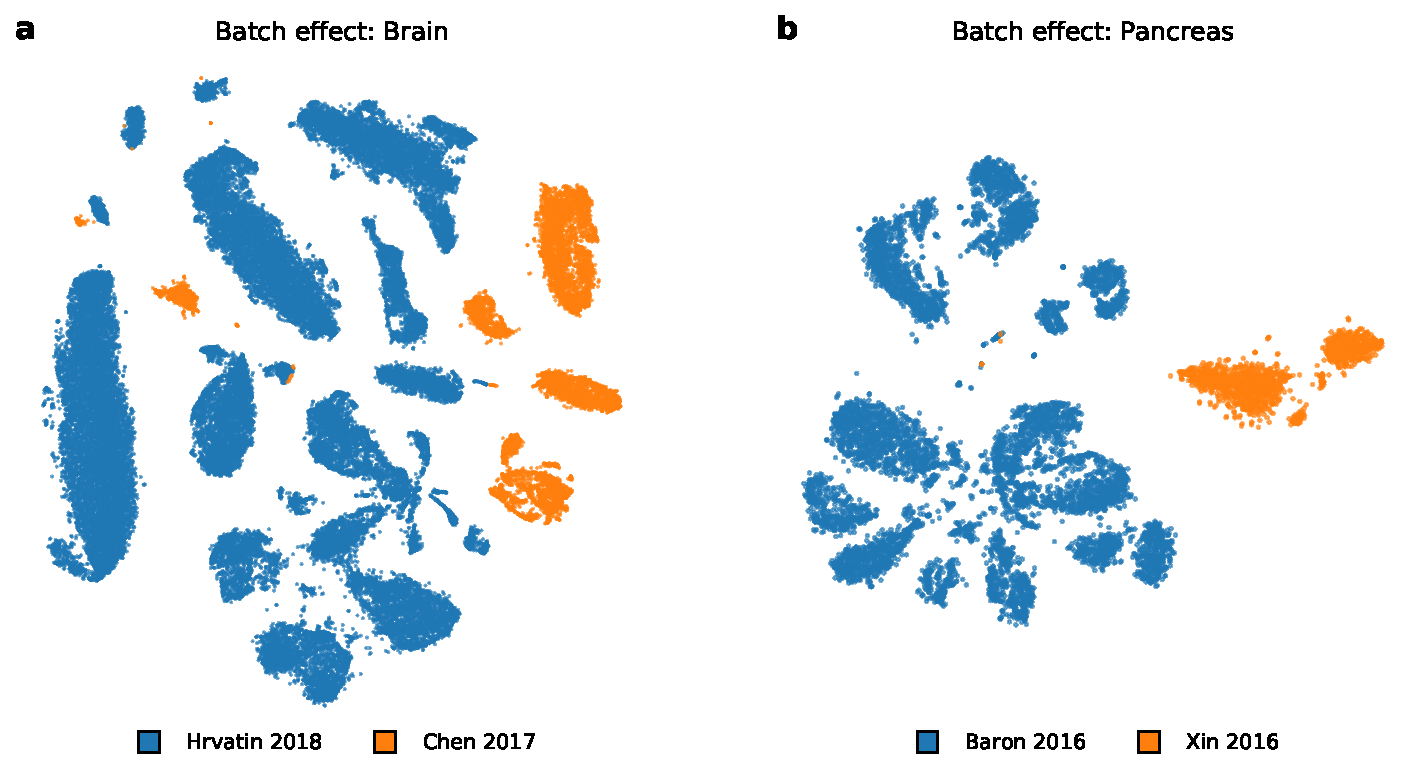
\includegraphics[width=\textwidth]{batch_effect.pdf}
  \caption{Batch effects are a driving factor of variation between the data
  sets. We depict a t-SNE visualization of two pairs of data sets. In each
  pair, the data sets share cell types, so we would expect cells
  from the reference data (blue) to mix with the cells in a secondary data
  sets (orange). Instead, t-SNE clusters data according to the
  data source.}
  \label{fig:batch_effect}
\end{figure}

Current solutions to embedding the data from various data sources address the
batch effect problems up-front. The data is typically preprocessed and
transformed such that the batch effects are explicitly removed. Recently
proposed procedures for batch effect removal include canonical correlation
analysis~\DIFdelbegin \DIFdel{\mbox{%DIFAUXCMD
\cite{cca} }\hspace{0pt}%DIFAUXCMD
}\DIFdelend \DIFaddbegin \DIFadd{\mbox{%DIFAUXCMD
\cite{Butler2018} }\hspace{0pt}%DIFAUXCMD
}\DIFaddend and mutual
nearest-neighbors~\DIFdelbegin \DIFdel{\mbox{%DIFAUXCMD
\cite{mnn,seurat}}\hspace{0pt}%DIFAUXCMD
}\DIFdelend \DIFaddbegin \DIFadd{\mbox{%DIFAUXCMD
\cite{Haghverdi2018,Stuart2019}}\hspace{0pt}%DIFAUXCMD
}\DIFaddend .  In these works, batch
effects are deemed removed when cells from different sources exhibit good mixing
in a t-SNE visualization. The elimination of batch effects may require
aggressive data preprocessing which may blur the boundaries between cell types.
Another problem is also the inclusion of any new data, for which the entire
analysis pipeline must be rerun, usually resulting in a different embedding
layout and clusters that have little resemblance to original visualization and
thus require reinterpretation.

We propose a direct solution of rendering t-SNE visualizations to address
batch effects. Our approach treats one of the data sets as a {\em reference}
and embeds the cells from another, {\em secondary data set} to a reference-defined
low-dimensional space.  We construct a t\nobreakdash -SNE embedding using the
reference data set, which is then used as a scaffold to embed the
secondary data. The key idea underpinning our approach is that secondary data
points are embedded independently of one another.

Independent embedding of each secondary datum causes the clustering landscape
to depend only on the reference scaffold, thus removing data source-driven
variation. In other words, when including new data, the scaffold inferred from
the reference data set is kept unchanged and defines a ``gravitational field'',
independently driving the embedding of each new instance. For example, in
Fig.~\ref{fig:transform_brain}, the cells from the visual cortex define the
scaffold (Fig.~\ref{fig:transform_brain}.a) into which we embed the cells from
the hypothalamus (Fig.~\ref{fig:transform_brain}.b). Unlike in their joint
t\nobreakdash -SNE visualization (Fig.~\ref{fig:batch_effect}.a), the
hypothalamic cells are dispersed across the entire embedding space and their
cell type correctly matches the prevailing type in reference clusters.

\begin{figure}[htb]
  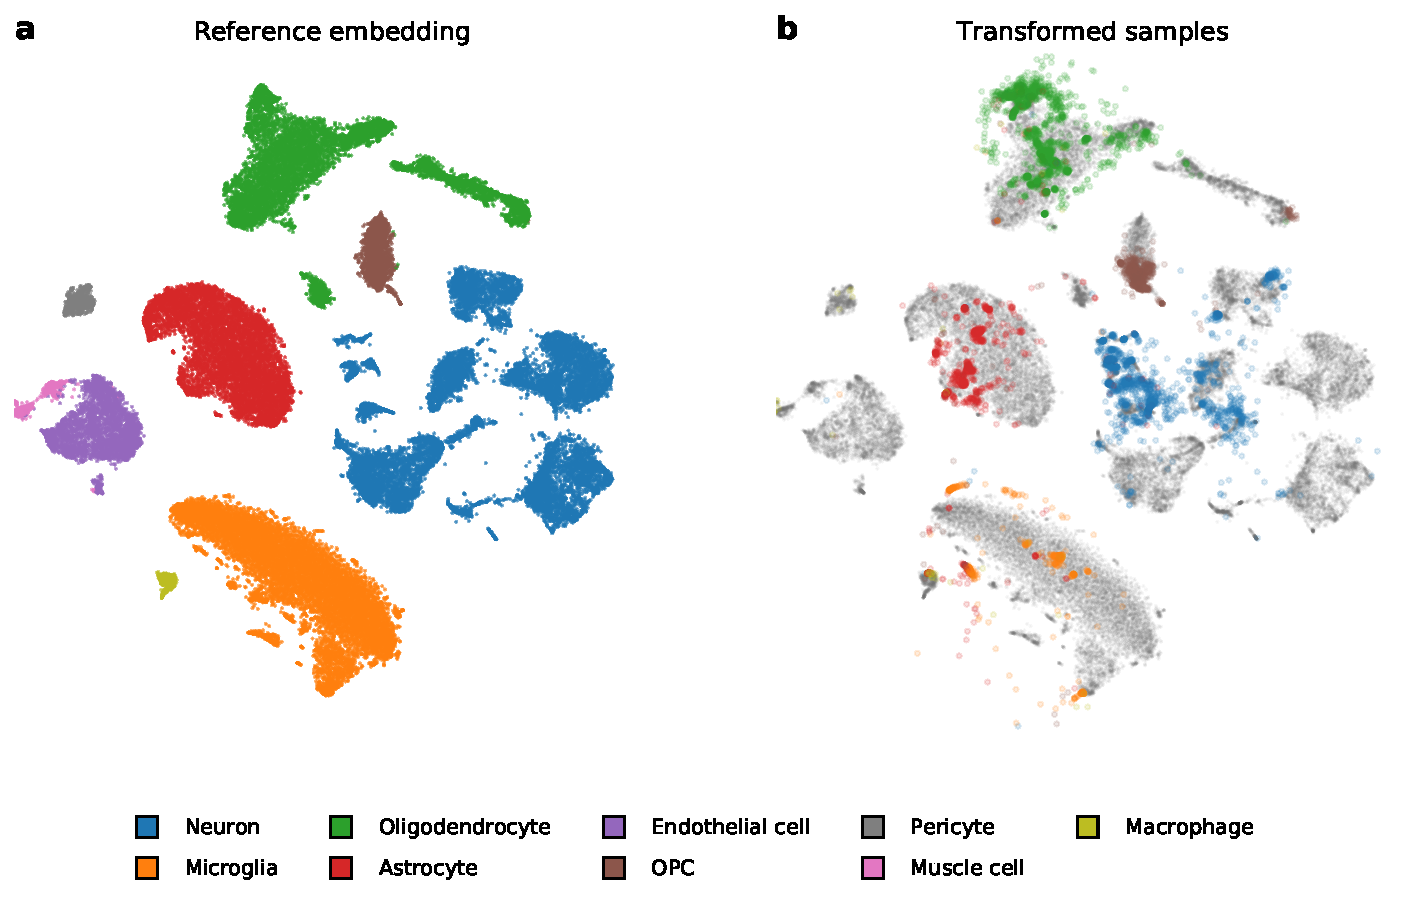
\includegraphics[width=\textwidth]{transform_brain.pdf}
  \caption{A two-dimensional embedding of a reference containing brain cells
  \textbf{(a)} and the corresponding mapping of secondary data containing hypothalamic
  cells \textbf{(b)}.  The majority of hypothalamic cells were mapped to their
  corresponding reference cluster. For instance, astrocyte cells marked with
  red on the right were mapped to an oval cluster of same-typed cells denoted
  with the same color in the visualization on the left.}
  \label{fig:transform_brain}
\end{figure}

The proposed solution implements a mapping of new data into an existing t-SNE
visualization. While the utility of such an algorithm was already hinted at in
recent publication~\DIFdelbegin \DIFdel{\mbox{%DIFAUXCMD
\cite{art_of_using_tsne}}\hspace{0pt}%DIFAUXCMD
}\DIFdelend \DIFaddbegin \DIFadd{\mbox{%DIFAUXCMD
\cite{Kobak2019}}\hspace{0pt}%DIFAUXCMD
}\DIFaddend , we here provide its practical and
theoretically-grounded implementation. Considering the abundance of recent
publications on batch effect removal, we present surprising evidence that a
computationally more direct and principled embedding procedure solves the batch
effects problem when constructing interpretable visualizations from different
data sources.


\DIFaddbegin \section{\DIFadd{Related Work}}

\DIFadd{Batch effects are systematic biases between biological data sets caused by
technical factors in the data collection and preparation process. It has been
well documented that even small differences in the experimental setup of
cell-dissociation, handling protocols, library-preparation technologies, or
sequencing platforms can significantly affect the resulting gene-expression
measurements~\mbox{%DIFAUXCMD
\cite{Tung2017,Hicks2018}}\hspace{0pt}%DIFAUXCMD
. When performing downstream comparative
analyses, batch effects may confound real biological variability and may
introduce spurious correlations, leading to misleading conclusions.
}

\DIFadd{Due to their severity, numerous computational approaches have been proposed to
directlty remove batch effects when performing joint analysis on two or more data sets.
Batch effect removal is typically performed as a preprocessing step. Existing
approaches involve either modifying the original data matrix or finding a joint
lower-dimensional space, where batch-effects are removed. Current methods
broadly fall into two categories: 1) mutual nearest neighbor based approaches
aim to identify matching populations of cells across the data sets, using them
to either find and correct the data sets~\mbox{%DIFAUXCMD
\cite{Haghverdi2018} }\hspace{0pt}%DIFAUXCMD
or directly
construct a batch-corrected k-nearest neighbor graph used in downstream
analyses~\mbox{%DIFAUXCMD
\cite{Park2018}}\hspace{0pt}%DIFAUXCMD
. 2) embedding multiple data sets into a joint
lower-dimensional space, where batch effects are removed. Some of these
approaches opt for linear dimensionality-reduction methods such as
PCA~\mbox{%DIFAUXCMD
\cite{Korsunsky2019} }\hspace{0pt}%DIFAUXCMD
or MultiCCA~\mbox{%DIFAUXCMD
\cite{Butler2018}}\hspace{0pt}%DIFAUXCMD
, while others employ
non-linear techniques from deep learning~\mbox{%DIFAUXCMD
\cite{Li2020,Lopez2018} }\hspace{0pt}%DIFAUXCMD
Still, other
approaches use a combination of the two~\mbox{%DIFAUXCMD
\cite{Stuart2019,Hie2019}}\hspace{0pt}%DIFAUXCMD
.
}

\DIFadd{Orthogonal approaches aimed at cell-type attempt to circumvent batch effects
altogether by identifying a subset of representative genes which act as markers
for a specific cell-type. Instead of considering the entire gene-expression
profile, which may be noisy and affected by batch effects, the idea is instead
to inspect the cells for the presence of a handful of genes, which could
adequately be used to determine the cell type. One such procedures is
scMap-Cluster, a consensus-based KNN method, tailored explicitly to scRNA-seq
gene-expression data~\mbox{%DIFAUXCMD
\cite{Kiselev2018}}\hspace{0pt}%DIFAUXCMD
. scMap-Cluster uses three
correlation-based distance measures and uses a voting scheme to perform
classification. To identify novel cell types, scMap-Cluster heuristically
determines a distance threshold.
}

\DIFadd{Broadly speaking, our approach falls into the second category, alongside
scMap-Cluster. The approach we describe uses standard single-cell pipelines
based on identifying representative genes. However, we emphasize that the
primary purpose of our approach is not classification, but the visualization of
the various cell-types. We can apply a KNN classifier to the resulting
visualizations to obtain accuracy estimates and compare our approach to other
classification methods. However, the classification aspect of our approach is
secondary: the primary purpose of t-SNE is to aid in scientists in exploratory
data analysis and help them better understand the underlying data landscape.
}


\DIFaddend \section{Methods}

We describe an end-to-end pipeline that uses fixed t-SNE coordinates as a
scaffold for embedding new (secondary) data, enabling joint visualization of
multiple data sources while mitigating batch effects. Our proposed approach
starts by using t\nobreakdash -SNE to embed a reference data set, with the aim
of constructing a two-dimensional visualization to facilitate interpretation
and cluster classification. Then, the placement of each new sample is optimized
independently via the t\nobreakdash -SNE loss function. Independent treatment
of each data instance from a secondary data set disregards any interactions
present in that data set, and prevents the formation of clusters that would be
specific to the secondary data. Below, we start with a summary of t-SNE and its
extensions (Sec.~\ref{sec:tsne}), introducing the relevant notation, upon which
we base our secondary data embedding approach (Sec.~\ref{sec:transfer}).


\subsection{Data Embedding by t-SNE and Its Extensions\label{sec:tsne}}

Local, non-linear dimensionality reduction by t-SNE is performed as follows.
Given a multi-dimensional data set $\mathbf{X} = \left \{ \mathbf{x}_1,
\mathbf{x}_2, \dots, \mathbf{x}_N \right \} \in \mathbb{R}^D$ where $N$ is the
number of data points in the reference data set, t-SNE aims to find a low
dimensional embedding $\mathbf{Y} = \left \{ \mathbf{y}_1, \mathbf{y}_2, \dots,
\mathbf{y}_N \right \} \in \mathbb{R}^d$ where $d \ll D$, such that if points
$\mathbf{x}_i$ and $\mathbf{x}_j$ are close in the multi-dimensional space,
their corresponding embeddings $\mathbf{y}_i$ and $\mathbf{y}_j$ are also
close. Since t-SNE is primarily used as a visualization tool, $d$ is typically
set to two. The similarity between two data points in t-SNE is defined as:

\begin{equation}
p_{j \mid i} = \frac{\exp \left ( -\frac{1}{2} \mathcal{D}(\mathbf{x}_i, \mathbf{x}_j ) / \sigma_i^2 \right )}{\sum_{k \neq i } \exp \left ( -\frac{1}{2} \mathcal{D}(\mathbf{x}_i, \mathbf{x}_k ) / \sigma_i^2 \right )}, \quad p_{i \mid i} = 0
\label{eq:gaussian_kernel}
\end{equation}

\noindent where $\mathcal{D}$ is a distance measure. This is then symmetrized to

\begin{equation}
p_{ij} = \frac{p_{j \mid i} + p_{i \mid j}}{2N}.
\label{eq:symmetrize}
\end{equation}

The bandwidth of each Gaussian kernel $\sigma_i$ is selected such that the
perplexity of the distribution matches a user-specified parameter value

\begin{equation}
\text{Perplexity} = 2^{H(P_i)}
\end{equation}

\noindent where $H(P_i)$ is the Shannon entropy of $P_i$,

\begin{equation}
H(P_i) = -\sum_i p_{j \mid i} \log_2 (p_{j \mid i}).
\end{equation}

\noindent Different bandwidths $\sigma_i$ enable t-SNE to adapt to the varying
density of the data in the multi-dimensional space.

The similarity between points $\mathbf{y}_i$ and $\mathbf{y}_j$ in the
embedding space is defined using the $t$-distribution with one degree of
freedom

\begin{equation}
q_{ij} = \frac{\left ( 1 + || \mathbf{y}_i - \mathbf{y}_j ||^2 \right )^{-1}}{\sum_{k \neq l}\left ( 1 + || \mathbf{y}_k - \mathbf{y}_l ||^2 \right )^{-1}},
\quad q_{ii} = 0.
\label{eq:cauchy_kernel}
\end{equation}

The t-SNE method finds an embedding $\mathbf{Y}$ that minimizes the
Kullback-Leibler (KL) divergence between $\mathbf{P}$ and $\mathbf{Q}$,

\begin{equation}
C = \text{KL}(\mathbf{P} \mid \mid \mathbf{Q}) = \sum_{ij} p_{ij} \log \frac{p_{ij}}{q_{ij}}.
\label{eq:kl_divergence}
\end{equation}

The time complexity needed to evaluate the similarities in
Eq.~\ref{eq:cauchy_kernel} is $\mathcal{O}(N^2)$, making its application
impractical for large data sets. We adopt a recent approach for low-rank
approximation of gradients based on polynomial interpolation which reduces its
time complexity to $\mathcal{O}(N)$. This approximation enables the
visualization of massive data sets, possibly containing millions of data
points~\DIFdelbegin \DIFdel{\mbox{%DIFAUXCMD
\cite{fi_tsne}}\hspace{0pt}%DIFAUXCMD
}\DIFdelend \DIFaddbegin \DIFadd{\mbox{%DIFAUXCMD
\cite{Linderman2019}}\hspace{0pt}%DIFAUXCMD
}\DIFaddend .

The resulting embeddings substantially depend on the value of the perplexity
parameter. Perplexity can be interpreted as the number of neighbors for which
the distances in the embedding space are preserved. Small values of perplexity
result in tightly-packed clusters of points and effectively ignore the
long-range interactions between clusters. Larger values may result in a more
globally consistent visualizations --- preserving distances on a large scale and
organizing clusters in a more meaningful way --- but can lead to merging small
clusters and thus obscuring local aspects of the data~\DIFdelbegin \DIFdel{\mbox{%DIFAUXCMD
\cite{art_of_using_tsne}}\hspace{0pt}%DIFAUXCMD
}\DIFdelend \DIFaddbegin \DIFadd{\mbox{%DIFAUXCMD
\cite{Kobak2019}}\hspace{0pt}%DIFAUXCMD
}\DIFaddend .

The trade-off between the local organization and global consistency may be
achieved by replacing the Gaussian kernels in Eq.~\ref{eq:gaussian_kernel} with
a mixture of Gaussians of varying bandwidths~\DIFdelbegin \DIFdel{\mbox{%DIFAUXCMD
\cite{multiscale_tsne}}\hspace{0pt}%DIFAUXCMD
}\DIFdelend \DIFaddbegin \DIFadd{\mbox{%DIFAUXCMD
\cite{Lee2015}}\hspace{0pt}%DIFAUXCMD
}\DIFaddend . Multi-scale kernels
are defined as

\begin{equation}
p_{j \mid i} \propto \frac{1}{L} \sum_{l=1}^{L} \exp \left ( - \frac{1}{2} \mathcal{D}(\mathbf{x}_i, \mathbf{x}_j ) / \sigma_{i,l}^2 \right ), \quad p_{i \mid i} = 0
\label{eq:multiscale}
\end{equation}

\noindent where $L$ is the number of mixture components. The bandwidths
$\sigma_{i,l}$ are selected in the same manner as in
Eq.~\ref{eq:gaussian_kernel}, but with a different value of perplexity for each
$l$. In our experiments, we used a mixture of two Gaussian kernels with
perplexity values of 50 and 500. A similar formulation of multi-scale kernels
was proposed in~\DIFdelbegin \DIFdel{\mbox{%DIFAUXCMD
\cite{art_of_using_tsne}}\hspace{0pt}%DIFAUXCMD
}\DIFdelend \DIFaddbegin \DIFadd{\mbox{%DIFAUXCMD
\cite{Kobak2019}}\hspace{0pt}%DIFAUXCMD
}\DIFaddend , and we found the resulting embeddings are
visually very similar to those obtained with the approach described above (not
shown for brevity).

When using t-SNE on larger data sets, the standard learning rate $\eta = 200$
has been shown to lead to slower convergence and requires more iterations to
achieve consistent embeddings~\DIFdelbegin \DIFdel{\mbox{%DIFAUXCMD
\cite{belkina2019automated}}\hspace{0pt}%DIFAUXCMD
}\DIFdelend \DIFaddbegin \DIFadd{\mbox{%DIFAUXCMD
\cite{Belkina2019}}\hspace{0pt}%DIFAUXCMD
}\DIFaddend . We follow the recommendation
of Belkina \etal ~and use a higher learning rate $\eta = N / 12$ when
visualizing larger data sets.


\subsection{Adding New Data Points to Reference Embedding\label{sec:transfer}}

Our algorithm, which embeds new data points to a reference embedding, consists
of estimating similarities between each new point and the reference data and
optimizing the position of each new data point in the embedding space. Unlike
parametric models such as principal component analysis or autoencoders, t-SNE
does not define an explicit mapping to the embedding space, and embeddings need
to be found through loss function optimization.

The position of a new data point in embedding space is initialized to the median
reference embedding position of its $k$ nearest neighbors. While we found the
algorithm to be robust to choices of $k$, we use $k=10$ in our experiments.

We adapt the standard t-SNE formulation from
Eqs.~\ref{eq:gaussian_kernel}~and~\ref{eq:cauchy_kernel} with

\begin{align}
p_{j \mid i} &= \frac{\exp \left ( -\frac{1}{2} \mathcal{D}(\mathbf{x}_i, \mathbf{v}_j) / \sigma_i^2 \right )}{\sum_{i} \exp \left ( -\frac{1}{2} \mathcal{D}(\mathbf{x}_i, \mathbf{v}_j) / \sigma_i^2 \right )}, \\
q_{j \mid i} &= \frac{\left ( 1 + || \mathbf{y}_i - \mathbf{w}_j ||^2 \right )^{-1}}{\sum_{i}\left ( 1 + || \mathbf{y}_i - \mathbf{w}_j ||^2 \right )^{-1}},
\end{align}

\noindent where $\mathbf{V} = \left \{ \mathbf{v}_1, \mathbf{v}_2, \dots,
\mathbf{v}_M \right \} \in \mathbb{R}^D$ where $M$ is the number of samples in
the secondary data set and $\mathbf{W} = \left \{ \mathbf{w}_1, \mathbf{w}_2, \dots,
\mathbf{w}_M \right \} \in \mathbb{R}^d$. Additionally, we omit the
symmetrization step in Eq.~\ref{eq:symmetrize}. This enables new points to be
inserted into the embedding independently of one another. The gradients of
$\mathbf{w}_j$ with respect to the loss (Eq.~\ref{eq:kl_divergence}) are:

\begin{equation}
\frac{\partial C}{\partial \mathbf{w}_j} = 2 \sum_i \left ( p_{j \mid i} - q_{j \mid i} \right ) \left ( \mathbf{y}_i - \mathbf{w}_j \right ) \left ( 1 + || \mathbf{y}_i - \mathbf{w}_j || ^2 \right )^{-1}
\label{eq:gradient}
\end{equation}

In the optimization step, we refine point positions using batch gradient
descent. We use an adaptive learning rate scheme with momentum to speed up the
convergence, as proposed by Jacobs~\DIFdelbegin \DIFdel{\mbox{%DIFAUXCMD
\cite{momentum,bh_tsne}}\hspace{0pt}%DIFAUXCMD
}\DIFdelend \DIFaddbegin \DIFadd{\mbox{%DIFAUXCMD
\cite{Jacobs1988,Maaten2014}}\hspace{0pt}%DIFAUXCMD
}\DIFaddend . We run gradient
descent with momentum $\alpha$ of $0.8$ for $250$ iterations, where the
optimization converged in all our experiments. The time complexity needed to
evaluate the gradients in Eq.~\ref{eq:gradient} is $\mathcal{O}(N \cdot M)$,
however, by adapting the same polynomial interpolation based approximation, this
is reduced to $\mathcal{O}(\max \{ N, M \})$. The time complexity can further be
reduced to $\mathcal{O}(M)$ by exploiting the fact that the reference embedding
remains fixed.

Special care must be taken to reduce the learning rate $\eta$ as the default
value in most implementations ($\eta = 200$) may cause points to ``shoot off''
from the reference embedding. This phenomenon is caused due to the embedding to
a previously defined t-SNE space, where the distances between data points and
corresponding gradients of the optimization function may be quite large. When
running standard t-SNE, points are initialized and scaled to have variance
0.0001. The resulting gradients tend to be very small during the initial phase,
resulting in stable convergence. When embedding new samples, the span of the
embedding is much larger, resulting in substantially larger gradients, and the
default learning rate causes points to move very far from the reference
embedding. In our experiments, we found that decreasing the learning rate to
$\eta \sim 0.1$ produces stable solutions. Alternatively, we can employ gradient
clipping to achieve similar behaviour. This is especially important when using
the interpolation-based approximation, which places a grid of interpolation
points over the embedding space, where the number of grid points is determined
by the span of the embedding. Clearly, if even one point ``shoots off'' far from
the embedding, the number of required grid points may grow dramatically,
increasing the runtime substantially. The reduced learning rate suppresses this
issue, and does not slow the convergence because of the adaptive learning rate
scheme, provided the optimization is run for a sufficient number of steps.

\section{Experiments and Discussion}

We apply the proposed approach to t-SNE visualizations of single-cell data. Data
in this realm include a variety of cells from specific tissues and are
characterized through gene expression.  In our experiments, we considered
several recently published data sets where cells were annotated with the cell
type. Our aim was to construct t-SNE visualizations where similarly-typed cells
would cluster together, despite systematic differences between data sources. To
that end, we focus on comparing different ways of using t-SNE rather than
differences to embeddings like PCA or MDS, which have been substantially covered
before~\DIFdelbegin \DIFdel{\mbox{%DIFAUXCMD
\cite{tsne,umap_single_cell}}\hspace{0pt}%DIFAUXCMD
}\DIFdelend \DIFaddbegin \DIFadd{\mbox{%DIFAUXCMD
\cite{Maaten2008,Becht2019}}\hspace{0pt}%DIFAUXCMD
}\DIFaddend . Below, we list the data sets \DIFdelbegin \DIFdel{,
describe single-cell specific data preprocessing procedures, }\DIFdelend \DIFaddbegin \DIFadd{used in our
experiments, }\DIFaddend and display the resulting data visualizations. \DIFaddbegin \DIFadd{Due to the unique
nature of single-cell data, we apply a specialized single-cell pipeline for all
our experiments, as described in Appendix~\ref{sec:sc-pipeline}. }\DIFaddend Finally, we
discuss the success of the proposed approach in alleviating the batch effects.


\subsection{Data}

We use three pairs of reference and secondary single-cell data sets originating
from different organisms and tissues. The data in each pair were chosen so that
the majority of cell types from the secondary data set were included in the
reference set (Table~\ref{tab:data sets}). The cells in the data sets originate
from the following three tissues:

\begin{description}
\item[Mouse brain.] The data set from Hrvatin \etal~\DIFdelbegin \DIFdel{\mbox{%DIFAUXCMD
\cite{hrvatin2018} }\hspace{0pt}%DIFAUXCMD
}\DIFdelend \DIFaddbegin \DIFadd{\mbox{%DIFAUXCMD
\cite{Hrvatin2018} }\hspace{0pt}%DIFAUXCMD
}\DIFaddend contains
cells from the visual cortex exploring transcriptional changes after exposure
to light. This was used as a reference for the data from Chen
\etal~\DIFdelbegin \DIFdel{\mbox{%DIFAUXCMD
\cite{chen2017}}\hspace{0pt}%DIFAUXCMD
}\DIFdelend \DIFaddbegin \DIFadd{\mbox{%DIFAUXCMD
\cite{Chen2017}}\hspace{0pt}%DIFAUXCMD
}\DIFaddend , containing cells from the mouse hypothalamus and
their reaction to food deprivation. From the secondary data, we removed cells
with no corresponding types in the reference: tanycytes, ependymal,
epithelial, and unlabelled cells.

\item[Human pancreas.] Baron \etal~\DIFdelbegin \DIFdel{\mbox{%DIFAUXCMD
\cite{baron2016} }\hspace{0pt}%DIFAUXCMD
}\DIFdelend \DIFaddbegin \DIFadd{\mbox{%DIFAUXCMD
\cite{Baron2016} }\hspace{0pt}%DIFAUXCMD
}\DIFaddend created
an atlas of pancreatic cell types. We used this set as a reference
for data from Xin \etal~\DIFdelbegin \DIFdel{\mbox{%DIFAUXCMD
\cite{xin2016}}\hspace{0pt}%DIFAUXCMD
}\DIFdelend \DIFaddbegin \DIFadd{\mbox{%DIFAUXCMD
\cite{Xin2016}}\hspace{0pt}%DIFAUXCMD
}\DIFaddend , who examined transcriptional
differences between healthy and type 2 diabetic patients.

\item[Mouse retina.] Macosko \etal~\DIFdelbegin \DIFdel{\mbox{%DIFAUXCMD
\cite{macosko2015} }\hspace{0pt}%DIFAUXCMD
}\DIFdelend \DIFaddbegin \DIFadd{\mbox{%DIFAUXCMD
\cite{Macosko2015} }\hspace{0pt}%DIFAUXCMD
}\DIFaddend created
an atlas of mouse retinal cell types. We used this as a reference
for the data from Shekhar \etal~\DIFdelbegin \DIFdel{\mbox{%DIFAUXCMD
\cite{shekhar2016}}\hspace{0pt}%DIFAUXCMD
}\DIFdelend \DIFaddbegin \DIFadd{\mbox{%DIFAUXCMD
\cite{Shekhar2016}}\hspace{0pt}%DIFAUXCMD
}\DIFaddend , who built an atlas for
retinal bipolar cells.
\end{description}

\vspace{-3mm}
\begin{table}[ht]
\begin{center}
\setlength\tabcolsep{4pt}
\begin{tabular}{l c c r c c}
\toprule
Study & Organism/Tissue & Protocol & Cells & Cell Types & Sparsity (\%) \\
\midrule
Hrvatin \etal & \multirow{2}{*}{mouse brain} & inDrop & 48,266 & 9 & 94 \\
Chen \etal & & Drop-seq & 14,437 & 6 & 93 \\[5pt]
Baron \etal & \multirow{2}{*}{human pancreas} & inDrop & 8,569 & 9 & 91 \\
Xin \etal & & SMARTer & 1,492 & 4 & 86 \\[5pt]
Macosko \etal & \multirow{2}{*}{mouse retina} & Drop-seq & 44,808 & 12 & 97 \\
Shekhar \etal & & Drop-seq & 27,499 & 5 & 96 \\
\bottomrule
\end{tabular}
\end{center}
\caption{Data sets used in our experiments. The first data set in each pair
(Hrvatin \etal, Baron \etal, and \DIFdelbeginFL \DIFdelFL{Macoscko }\DIFdelendFL \DIFaddbeginFL \DIFaddFL{Macosko }\DIFaddendFL \etal) was used as a reference.  We
relied on the quality control and annotations from the original publication
and report the number of cell types after preprocessinng.  The cell
annotations were made consistent to annotations from the Cell
Ontology~\DIFdelbeginFL \DIFdelFL{\mbox{%DIFAUXCMD
\cite{cell_ontology}}\hspace{0pt}%DIFAUXCMD
}\DIFdelendFL \DIFaddbeginFL \DIFaddFL{\mbox{%DIFAUXCMD
\cite{Bard2005}}\hspace{0pt}%DIFAUXCMD
}\DIFaddendFL . Notice that different RNA sequencing protocols
were used to estimate gene expressions.}
\label{tab:data sets}
\end{table}

\subsection{\DIFdelbegin \DIFdel{Results and Discussion}\DIFdelend \DIFaddbegin \DIFadd{t-SNE transform successfully alleviates batch effects}\DIFaddend }
\label{sec:results}

Figs.~\ref{fig:transform_brain}, \ref{fig:transform_pancreas}, and
\ref{fig:transform_retina} show the embeddings of the reference data sets and
their corresponding embeddings of the secondary data sets. In all the figures,
the cells from the secondary data sets were positioned in the cluster of
same-typed reference cells, providing strong evidence of the success of our approach. There are some deviations to these observations; for
instance, in Fig.~\ref{fig:transform_brain} several oligodendrocyte precursor
cells (OPCs) were mapped to oligodendrocytes. This may be due to differences in
annotation criteria by different authors, or due to inherent similarities of
these types of cells. Examples of such erroneous placements can be found in
other figures as well, but are uncommon and constitute less then 5\% of
the cells (less than 5\% in brain, 1\% in pancreas and 2\% in retina
secondary data).

Notice that we could simulate the split between reference and secondary data
sets using one data set only and perform cross-validation, however this type of
experiment would not incorporate batch effects. We want to remind the reader
that handling batch effects were central to our endeavour and that the
disregard of this effect could lead to overly-optimistic results and data
visualizations strikingly different from ours. For example, compare the
visualizations from Fig.~\ref{fig:batch_effect}.a and
Fig.~\ref{fig:transform_brain}.b, or Figs.~\ref{fig:batch_effect}.b and
\ref{fig:transform_pancreas}.b.


\begin{figure}[htb]
  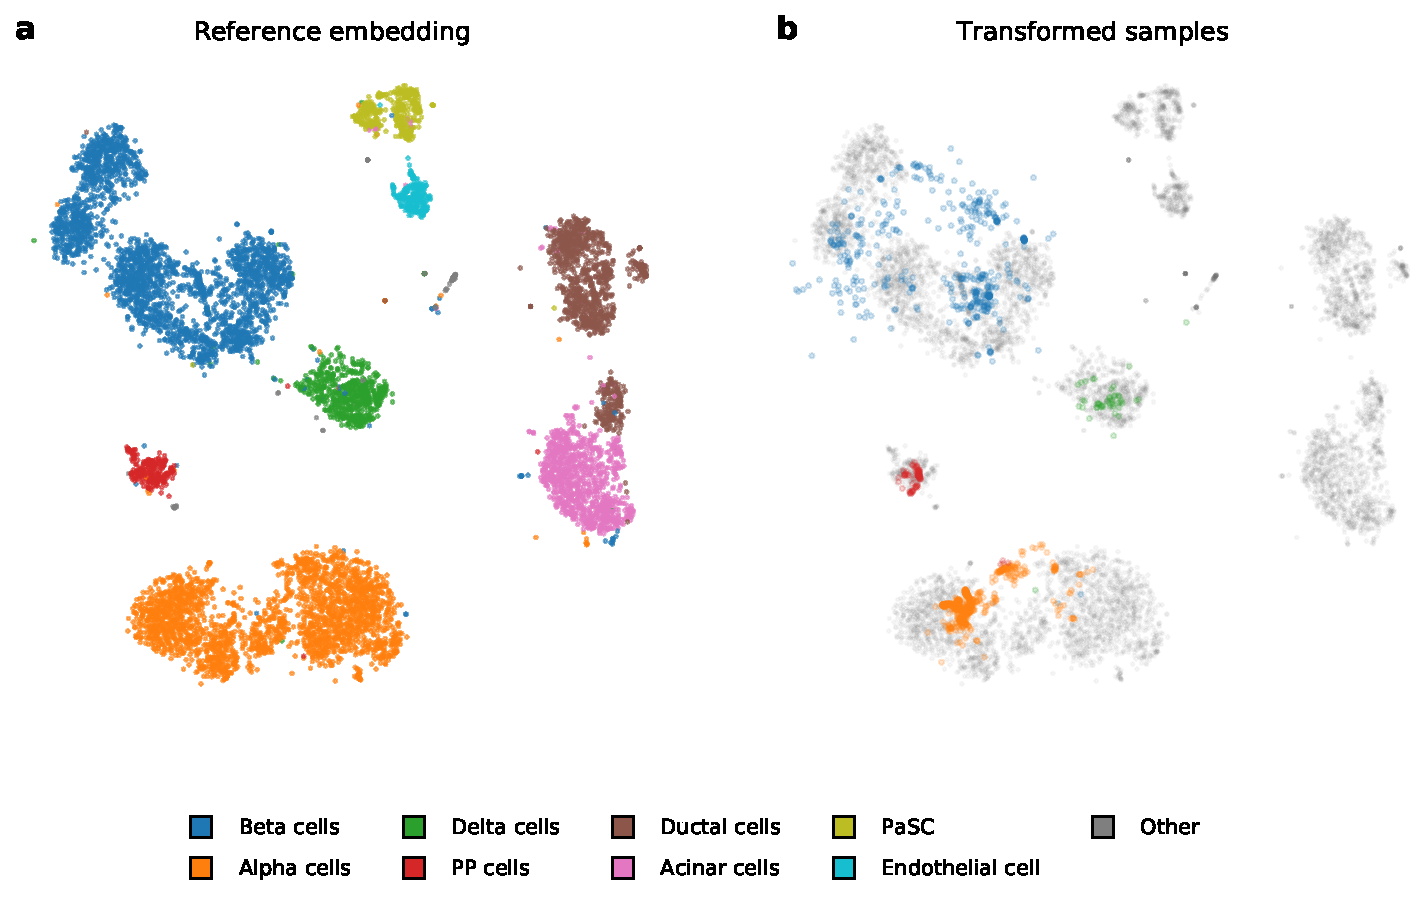
\includegraphics[width=\textwidth]{transform_pancreas.pdf}
  \caption{Embedding of pancreatic cells from Baron \etal~\DIFdelbeginFL \DIFdelFL{\mbox{%DIFAUXCMD
\cite{baron2016} }\hspace{0pt}%DIFAUXCMD
}\DIFdelendFL \DIFaddbeginFL \DIFaddFL{\mbox{%DIFAUXCMD
\cite{Baron2016} }\hspace{0pt}%DIFAUXCMD
}\DIFaddendFL and
  cells from the same tissue from Xin \etal~\DIFdelbeginFL \DIFdelFL{\mbox{%DIFAUXCMD
\cite{xin2016}}\hspace{0pt}%DIFAUXCMD
}\DIFdelendFL \DIFaddbeginFL \DIFaddFL{\mbox{%DIFAUXCMD
\cite{Xin2016}}\hspace{0pt}%DIFAUXCMD
}\DIFaddendFL . Just like in
  Fig.~\ref{fig:transform_brain}, the vast majority of the cells from the
  secondary data set were correctly mapped to the same-typed cluster of
  reference cells.}
  \label{fig:transform_pancreas}
\end{figure}


\begin{figure}[htb]
  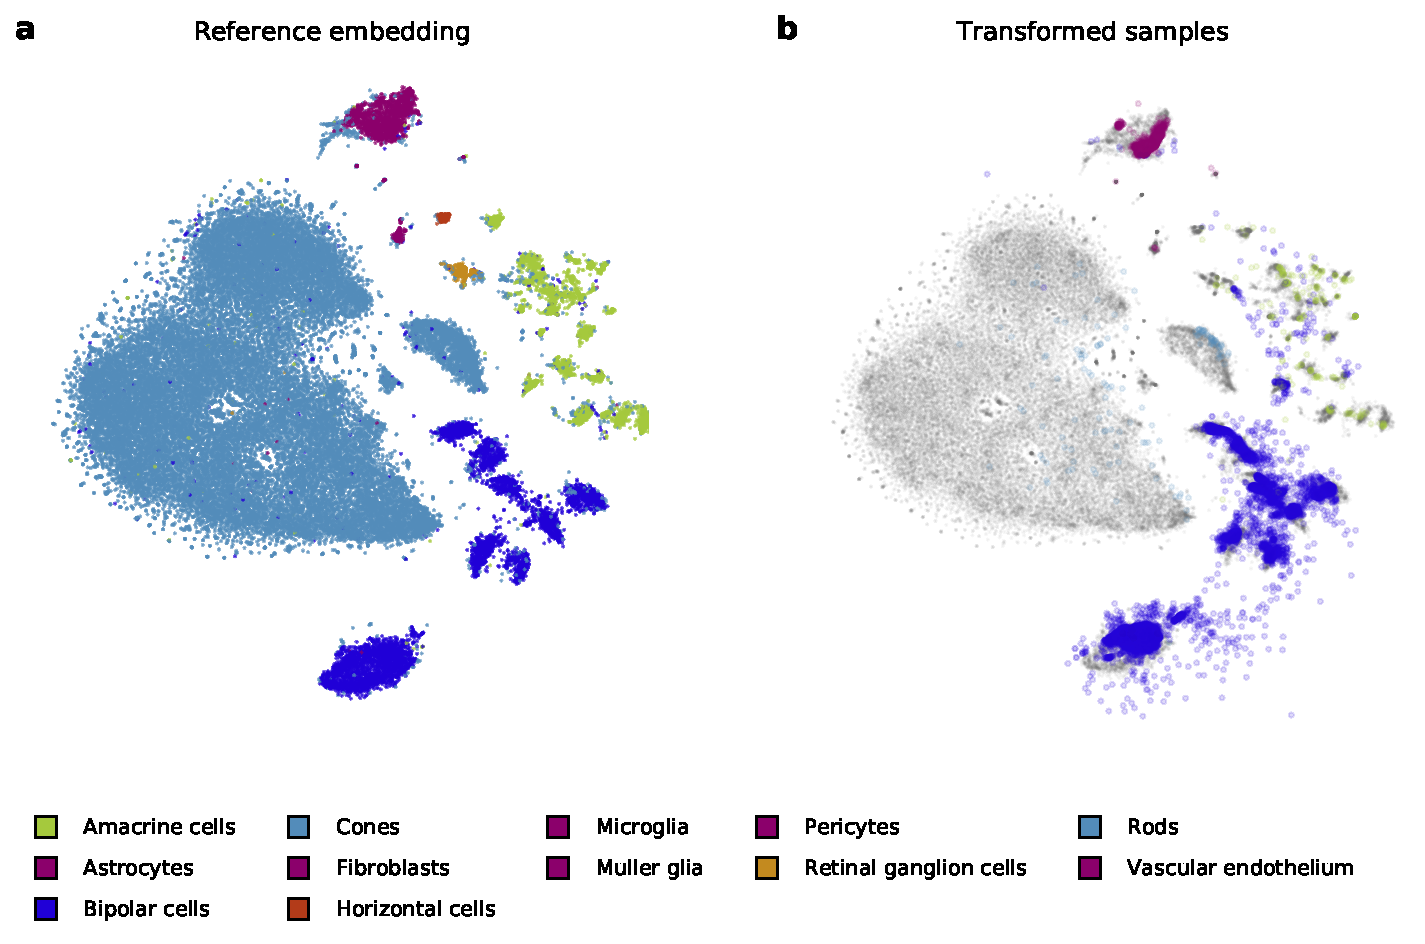
\includegraphics[width=\textwidth]{transform_retina.pdf}
  \caption{An embedding of a large reference of retinal cells from Macosco
  \etal~\DIFdelbeginFL \DIFdelFL{\mbox{%DIFAUXCMD
\cite{macosko2015} }\hspace{0pt}%DIFAUXCMD
}\DIFdelendFL \DIFaddbeginFL \DIFaddFL{\mbox{%DIFAUXCMD
\cite{Macosko2015} }\hspace{0pt}%DIFAUXCMD
}\DIFaddendFL \textbf{(a)} and mapping of cells from a smaller study that
  focuses on bipolar cells from Shekhar \etal~\DIFdelbeginFL \DIFdelFL{\mbox{%DIFAUXCMD
\cite{shekhar2016} }\hspace{0pt}%DIFAUXCMD
}\DIFdelendFL \DIFaddbeginFL \DIFaddFL{\mbox{%DIFAUXCMD
\cite{Shekhar2016} }\hspace{0pt}%DIFAUXCMD
}\DIFaddendFL \textbf{(b)}. We use
  colors consistent with the study by Macosko \etal}
  \label{fig:transform_retina}
\end{figure}


\DIFaddbegin \subsection{\DIFadd{Constructing a reference embedding}}

\DIFaddend We use a number of additional, recently proposed modifications to enhance the t-SNE visualization of the reference data set.
Kobak and Linderman have shown that the global consistency of embeddings produced by
popular visualization algorithms are largely dependent on their initialization~\DIFdelbegin \DIFdel{\mbox{%DIFAUXCMD
\cite{kobak2019umap}}\hspace{0pt}%DIFAUXCMD
}\DIFdelend \DIFaddbegin \DIFadd{\mbox{%DIFAUXCMD
\cite{Kobak2019a}}\hspace{0pt}%DIFAUXCMD
}\DIFaddend . By utilizing PCA-based initialization, t-SNE is able to achieve
more meaningful layouts of the resulting clusters (Fig.~\ref{fig:multiscale}.b)
as opposed to using randomly initialized embeddings (Fig.~\ref{fig:multiscale}.a).
Another important extension is the use of multi-scale similarities, which, in addition
to considering short range interactions, also models wider point neighborhoods. Coupled
with PCA-based initializations, this produces even more meaningful visualizations where
clusters form interpretable structures. For instance, consider Fig.~\ref{fig:multiscale}.c, which reveals two meaningful subgroups of GABAergic neurons, corresponding to their
developmental origin, as discussed in Tasic \etal~\DIFdelbegin \DIFdel{\mbox{%DIFAUXCMD
\cite{tasic2018}}\hspace{0pt}%DIFAUXCMD
}\DIFdelend \DIFaddbegin \DIFadd{\mbox{%DIFAUXCMD
\cite{Tasic2018}}\hspace{0pt}%DIFAUXCMD
}\DIFaddend , while this division
is less apparent when using PCA-based initialization alone in
Fig.~\ref{fig:multiscale}.b.

We also observed the important role of gene selection in crafting the reference
embedding spaces. We found that when selecting an insufficient number of genes,
the resulting visualizations display overly-fragmented clusters. When the
selection is too broad and includes lowly expressed genes, the subclusters tend
to overlap. These effects can all be attributed to sparseness of the data sets
and may be intrinsic to single-cell data. In our studies, we found that
selection of 3,000 genes yields most informative visualizations
(Fig.~\ref{fig:gene_selection}).

\DIFaddbegin \subsection{\DIFadd{Optimization is crucial to producing meaningful point embeddings}}

\DIFaddend In principle, our theoretically-grounded embedding of secondary data into the
scaffold defined by the reference embedding could be simplified with the
application of the nearest neighbors-based procedure. For example, while
describing a set of tricks for t-SNE, Kobak and Berens~\DIFdelbegin \DIFdel{\mbox{%DIFAUXCMD
\cite{art_of_using_tsne}
}\hspace{0pt}%DIFAUXCMD
}\DIFdelend \DIFaddbegin \DIFadd{\mbox{%DIFAUXCMD
\cite{Kobak2019}
}\hspace{0pt}%DIFAUXCMD
}\DIFaddend proposed positioning new points into a known embedding by placing them in the
median position of their 10 nearest neighbors, where the neighborhood was
estimated in the original data space. Notice that we use this approach as well,
but only for the initialization of positions of new data instances that are
subject to further optimization. Despite both nearest-neighbors search and
t-SNE optimization can be computed in linear time, the former dominates the
runtime (mouse retina example; 44,808 reference, 26,830 secondary cells,
9min NN-search, 13sec optimization).

Fig.~\ref{fig:optimization} demonstrates a case where nearest neighbor-based 
positioning alone is insufficient. We construct a reference embedding using only
neurons from Hrvatin \etal~\DIFdelbegin \DIFdel{\mbox{%DIFAUXCMD
\cite{hrvatin2018} }\hspace{0pt}%DIFAUXCMD
}\DIFdelend \DIFaddbegin \DIFadd{\mbox{%DIFAUXCMD
\cite{Hrvatin2018} }\hspace{0pt}%DIFAUXCMD
}\DIFaddend (Fig.~\ref{fig:optimization}.a)
and use that to position neuronal
cells from the data set from Campbell \etal~\DIFdelbegin \DIFdel{\mbox{%DIFAUXCMD
\cite{campbell2017}}\hspace{0pt}%DIFAUXCMD
}\DIFdelend \DIFaddbegin \DIFadd{\mbox{%DIFAUXCMD
\cite{Campbell2017}}\hspace{0pt}%DIFAUXCMD
}\DIFaddend . We utilize the
weighted mean and median positions to initialize point positions from the secondary
data set, as shown in Figs.~\ref{fig:optimization}.b and \ref{fig:optimization}.c.
After initialization, we optimize point positions using the procedure described
above for 500 iterations. The resulting visualizations from both initializations
are visually very similar, indicating stable convergence. We show one of the resulting
visualizations in Fig.~\ref{fig:optimization}.b.

Notice that both neighbor-based initialization schemes generally position data points
such that their classification is unclear. Median-based initialization produces
a sort of grid-like structure, while median based initialization positions the points
almost continuously across the embedding space. Optimization reveals strong
correspondence of several points to reference-defined clusters, while other points
from the secondary data set are pushed away from their initial clusters, possibly
indicating dissimilarity.


\begin{figure}[htbp]
  \includegraphics[width=\textwidth]{optimization.pdf}
  \caption{Comparison of different initialization schemes for positioning new data
  points onto reference embeddings. {\bf (a)} We construct a reference embedding
  using only neuronal subtypes from Hrvatin \etal~\DIFdelbeginFL \DIFdelFL{\mbox{%DIFAUXCMD
\cite{hrvatin2018}}\hspace{0pt}%DIFAUXCMD
}\DIFdelendFL \DIFaddbeginFL \DIFaddFL{\mbox{%DIFAUXCMD
\cite{Hrvatin2018}}\hspace{0pt}%DIFAUXCMD
}\DIFaddendFL . {\bf (b)}
  We position neuronal cells from Campbell \etal~\DIFdelbeginFL \DIFdelFL{\mbox{%DIFAUXCMD
\cite{campbell2017} }\hspace{0pt}%DIFAUXCMD
}\DIFdelendFL \DIFaddbeginFL \DIFaddFL{\mbox{%DIFAUXCMD
\cite{Campbell2017} }\hspace{0pt}%DIFAUXCMD
}\DIFaddendFL using the
  median initizaliation scheme from Kobak and Berens~\DIFdelbeginFL \DIFdelFL{\mbox{%DIFAUXCMD
\cite{art_of_using_tsne} }\hspace{0pt}%DIFAUXCMD
}\DIFdelendFL \DIFaddbeginFL \DIFaddFL{\mbox{%DIFAUXCMD
\cite{Kobak2019} }\hspace{0pt}%DIFAUXCMD
}\DIFaddendFL and
  run optimization for 500 iterations. Compare the optimized embedding with the 
  initial median initialization {\bf (c)} or by using a simple weighted mean
  initialization {\bf (d)}.}
  \label{fig:optimization}
\end{figure}

\DIFdelbegin \DIFdel{The }\DIFdelend \DIFaddbegin \subsection{\DIFadd{Our approach requires a complete reference set}}

\DIFadd{Our }\DIFaddend approach assumes that all cell types from the secondary data set are present
in the reference. \DIFaddbegin \DIFadd{Intuitively, using t-SNE in such a way is conceptually similar
to classification via $k$-nearest neighbor classifiers and is similarily
limited. }\DIFaddend The method may fail to reveal \DIFdelbegin \DIFdel{novel }\DIFdelend \DIFaddbegin \DIFadd{unseen }\DIFaddend cell types in the secondary data
set, \DIFdelbegin \DIFdel{possibly }\DIFdelend \DIFaddbegin \DIFadd{likely }\DIFaddend positioning them arbitrarily close to unrelated clusters. \DIFdelbegin \DIFdel{Procedures such as scmap were recently proposed to cope
with such cases and identify the cells whose type is new and not included in
the reference~\mbox{%DIFAUXCMD
\cite{scmap}}\hspace{0pt}%DIFAUXCMD
}\DIFdelend \DIFaddbegin \DIFadd{In some
instances, unknown cell types may be sufficiently different from the reference
data that t-SNE will repel them from existing clusters. However, we caution that
this approach is unreliable and depends heavily on the chosen preprocessing
pipeline.
}

\DIFadd{We illustrate this with Fig.~\ref{fig:incomplete_reference}, where we first fit
create a reference embedding containing only neuronal cells from Hrvatin
\etal~\mbox{%DIFAUXCMD
\cite{Hrvatin2018}}\hspace{0pt}%DIFAUXCMD
. We then select only non-neuronal cells from Campbell
\etal~\mbox{%DIFAUXCMD
\cite{Campbell2017} }\hspace{0pt}%DIFAUXCMD
and add them to the reference embedding in
Fig.~\ref{fig:incomplete_reference}.b. The non-neuronal cells from Hrvatin \etal
are scattered somewhat arbitrarily around several clusters in the reference
embedding. Interestingly, the secondary data points form a ``ring'' around one
of the clusters, indicating that these data points are very different from the
cells in this cluster. Notice also that the points from the secondary data set
exhibit little to no clustering and the different cell types seem to be mixed
amongst each other. We hypothesize that this effect is due primarily to the
single-cell preprocessing pipeline and not the limitations of our proceedure
itself, as the informative genes selected to create the reference neuronal
embedding likely do not differentiate supportive glial cells from the secondary
data set. This effect is similar to procedures such as scMap-Cluster, a consensus KNN
method, which heuristically determines a distance threshold to identify unknown
cell types~\mbox{%DIFAUXCMD
\cite{Kiselev2018}}\hspace{0pt}%DIFAUXCMD
}\DIFaddend .

\DIFaddbegin \begin{figure}[htb]
  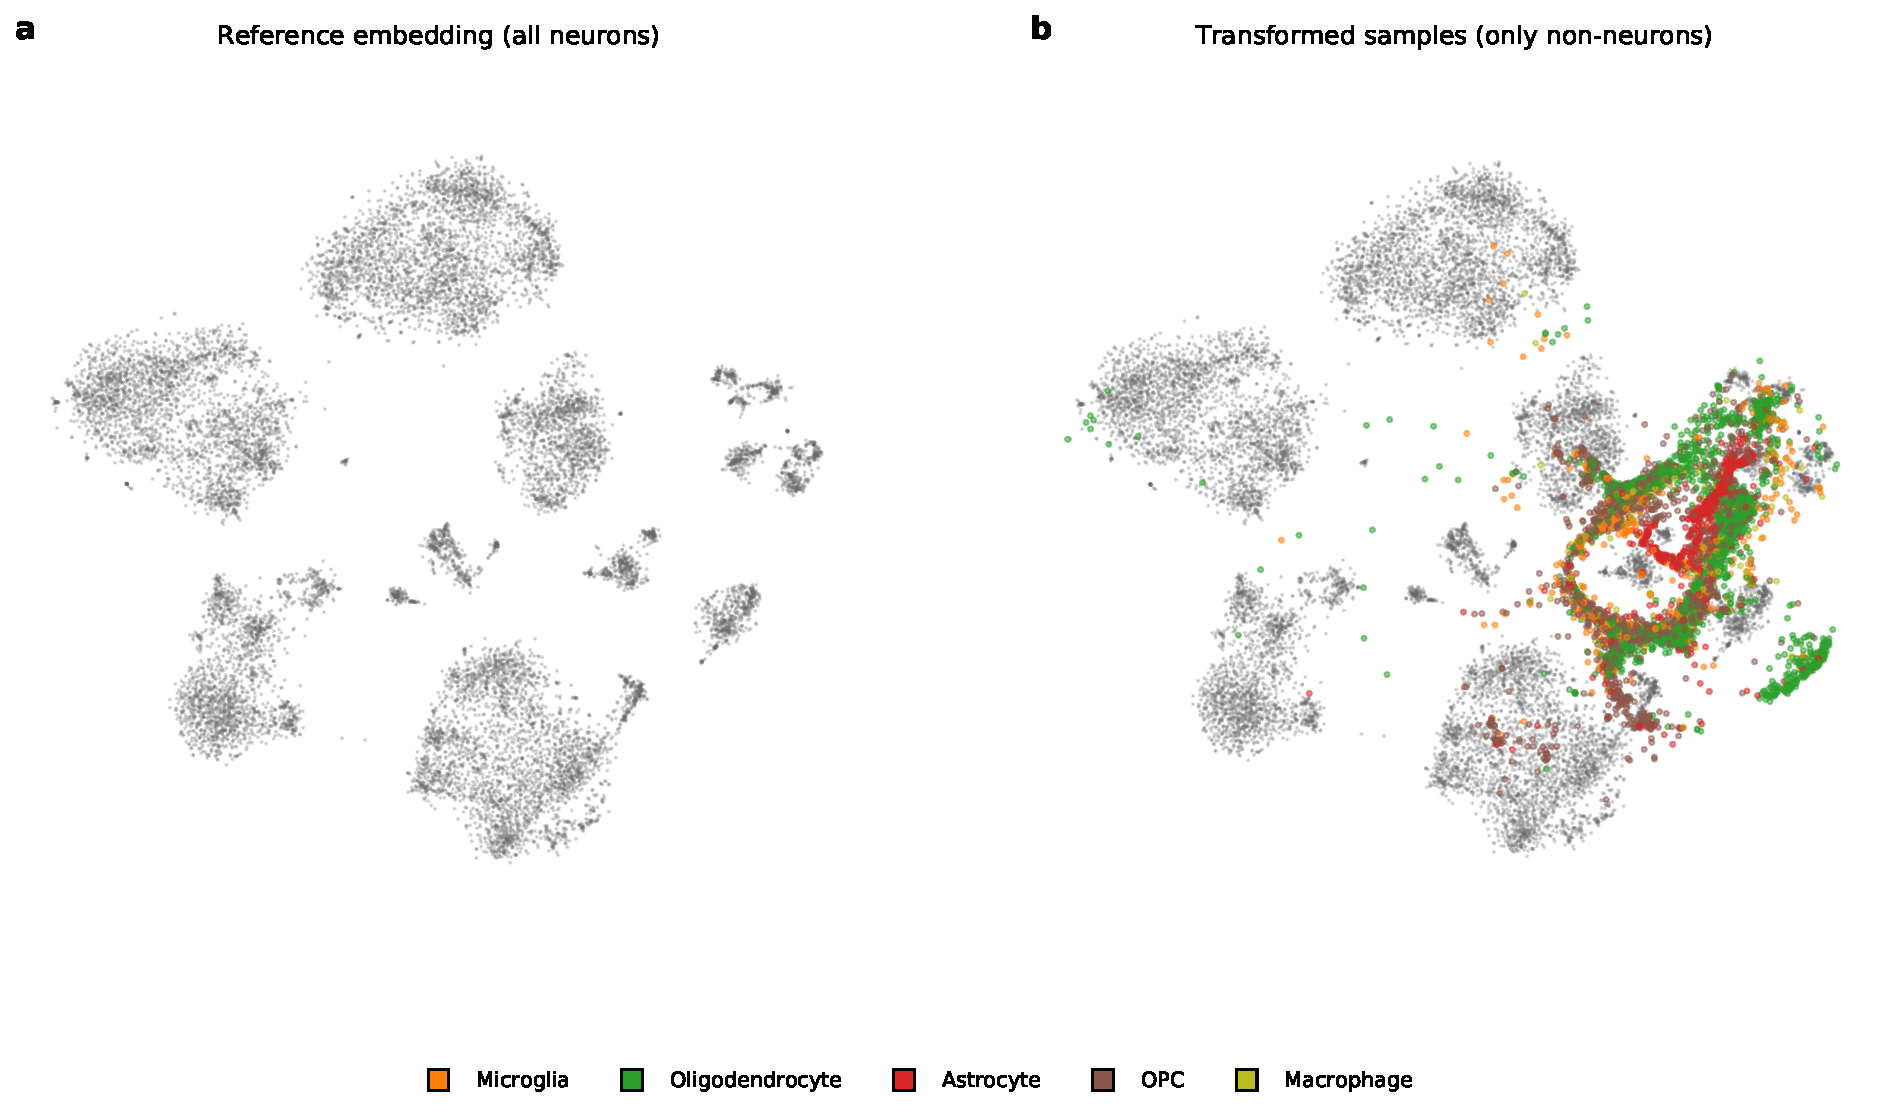
\includegraphics[width=\textwidth]{incomplete_reference-brain.pdf}
  \caption{\DIFaddFL{A reference embedding must contain all the cell-types in the
  secondary embedding to produce reliable results. }{\bf \DIFaddFL{(a)}} \DIFaddFL{We construct a
  reference embedding containing only neuronal cells from Hrvatin
  \etal~\mbox{%DIFAUXCMD
\cite{Hrvatin2018}}\hspace{0pt}%DIFAUXCMD
. }{\bf \DIFaddFL{(b)}} \DIFaddFL{We select only non-neuronal cells from
  Campbell \etal~\mbox{%DIFAUXCMD
\cite{Campbell2017} }\hspace{0pt}%DIFAUXCMD
so that no overlap exists between the
  cell-types between the data sets. Conceptually, t-SNE behaves similarily to a
  KNN classifier, and places the non-neurnal cells to their the most similar
  points in the reference. In some instances, the non-neuronal cells are
  sufficiently different from the neuronal cells so that they are repelled from
  the reference clusters. Such behaviour results in the ``ring'' seen on the
  right hand side of the embedding.}} \label{fig:incomplete_reference}
\end{figure}

\DIFaddend Our procedure is, therefore, asymmetrical in the choice of reference and
secondary data set. In practice, however, newly produced {\em secondary} data
would be embedded into previously-prepared reference landscapes. Large
collections of data {\em e.g.} the Human Cell Atlas
initiative~\DIFdelbegin \DIFdel{\mbox{%DIFAUXCMD
\cite{hca} }\hspace{0pt}%DIFAUXCMD
}\DIFdelend \DIFaddbegin \DIFadd{\mbox{%DIFAUXCMD
\cite{Rozenblatt-Rosen2017} }\hspace{0pt}%DIFAUXCMD
}\DIFaddend make it possible to scale up our approach
to wider sets of cell types. \DIFaddbegin \DIFadd{Identifying potential failure cases where rare
cell-types may still be missing from constructed reference embeddings is a
problem that plagues the bioinformatics community and is an active area of
research.
}\DIFaddend 


\DIFaddbegin \subsection{\DIFadd{Comparison to other similar batch-effect methods}}

\DIFaddend To quantitatively evaluate the predictive accuracy of the described procedure,
we fit $k$-nearest neighbors classifiers on each reference t-SNE embedding from
Figs.~\ref{fig:transform_brain}.a, \ref{fig:transform_pancreas}.a and
\ref{fig:transform_retina}.a and use them to predict the cell types for the
secondary data set embeddings from Figs.~\ref{fig:transform_brain}.b,
\ref{fig:transform_pancreas}.b and \ref{fig:transform_retina}.b. The accuracy
measures are reported in Table~\ref{tab:scores}. Our procedure of embedding new
data points into two-dimensional t-SNE plane results in similar accuracy to
approaches like random forests that use full compendium of cell-characterizing
features. The results indicate that positioning of new cells onto a cell
visualisation plane is not only indicative but also an accurate instrument for
cell type characterization.

\begin{table}[ht]
\centering
  \setlength\tabcolsep{6pt}
  \begin{tabular}{c c r r}
  \toprule
  Tissue & Method & Accuracy & ARI \\
  \toprule
  \multirow{4}{*}{mouse brain} & t-SNE & 0.96 & 0.93 \\
   & KNN & 0.96 & 0.93 \\
   & Random Forest & \textbf{0.98} & \textbf{0.96} \\
   & scMap-Cluster & 0.66 & 0.70 \\
  \midrule
  \multirow{4}{*}{human pancreas} & t-SNE & \textbf{0.99} & \textbf{0.99} \\
   & KNN & \textbf{0.99} & 0.98 \\
   & Random Forest & 0.96 & 0.89 \\
   & scMap-Cluster & 0.95 & 0.93 \\
  \midrule
  \multirow{4}{*}{mouse retina} & t-SNE & \textbf{0.99} & 0.94 \\
   & KNN & \textbf{0.99} & 0.96 \\
   & Random Forest & \textbf{0.99} & \textbf{0.99} \\
   & scMap-Cluster & 0.88 & 0.59 \\
  \bottomrule
  \end{tabular}
  \caption{We compare our approach (t-SNE) to three other methods, evaluating
    performance using classification accuracy and the adjusted rand index (ARI).
    Notice that while the proposed approach classifies cells only based on their
    position on the two-dimensional plane, it performs comparably to other
    methods that use full compendium of features (gene expressions) that
    characterize the cells.}
  \label{tab:scores}
\end{table}

We compare our approach to two machine learning techniques, namely a $k$-nearest
neighbor classifier (KNN) and a random forest ensemble, and
scMap-Cluster~\DIFdelbegin \DIFdel{\mbox{%DIFAUXCMD
\cite{scmap}}\hspace{0pt}%DIFAUXCMD
, a $k$-nearest neighbor based method, tailored explicitly to scRNA-seq data. }\DIFdelend \DIFaddbegin \DIFadd{\mbox{%DIFAUXCMD
\cite{Kiselev2018}}\hspace{0pt}%DIFAUXCMD
. For }\DIFaddend scMap-Cluster\DIFdelbegin \DIFdel{uses three correlation-based distance
measures and uses a voting scheme to perform classification. A threshold may also be set so that new cell typesmay be labeled as }%DIFDELCMD < {\tt %%%
\DIFdel{unrecognized}%DIFDELCMD < }%%%
\DIFdel{, but since }\DIFdelend \DIFaddbegin \DIFadd{, we disable the distance
threshold heuristic for identifying novel cell types, as }\DIFaddend our secondary data sets
were chosen such that \DIFdelbegin \DIFdel{this does not happen, this was disabled}\DIFdelend \DIFaddbegin \DIFadd{there is complete overlap between cell-types}\DIFaddend . For the two
machine learning approaches, we apply the typical single-cell preprocessing
pipeline described in \DIFdelbegin \DIFdel{Sec.}\DIFdelend \DIFaddbegin \DIFadd{Appendix}\DIFaddend ~\ref{sec:sc-pipeline}, i.e., library-size
normalization, log-transformation, and select 1,000 most informative genes.
Similarily to scMap-Cluster, we use the cosine distance to find the 5 nearest
neighbors in the KNN model. We used 100 trees in the random forest ensemble. The
models were fit on the reference data set, and no hyper-parameter tuning was
performed.

Surprisingly, both the random forest and $k$-nearest neighbor models outperform
scMap-Cluster, which is specifically tailored to scRNA-seq data. However, these
results may be skewed, as, in our examples, all the cell-types from the
secondary data set were present in the reference data set. One of the core
features of scMap-Cluster is the detection of novel cell types, which none of
the other methods support. In other words, the other three methods would always
assign a cell-type to a given cell, regardless of cell origin. Additionally,
scMap-Cluster was primarily designed and tested on data sets produced by
full-length sequencing protocols, which tend to detect a much higher number of
molecules than other, sequencing protocols based on unique molecular identifiers
(UMI). These two classes of sequencing protocols produce data sets with
different sparsity and variance characteristics. This is consistent with the
results in Table~\ref{tab:scores}, as only the data sets from the human
pancreas, were produced using a full-length sequencing protocol, where
scMap-Cluster achieves reasonably high accuracy.

The aim of t-SNE is to construct embeddings, in which neighborhoods are
preserved, therefore it is unsurprising that the accuracy of our t-SNE based
approach is largely consistent with the $k$-nearest neighbors model. \DIFdelbegin \DIFdel{Our }\DIFdelend \DIFaddbegin \DIFadd{While our
}\DIFaddend approach is comparable to the other models in terms of accuracy, \DIFdelbegin \DIFdel{but we would note }\DIFdelend \DIFaddbegin \DIFadd{we emphasize
}\DIFaddend that the goal of t-SNE embeddings is to serve as visual aids in exploratory data
analysis. \DIFdelbegin \DIFdel{However, our procedure, }\DIFdelend \DIFaddbegin \DIFadd{Therefore, it is surprising that our simple procedure performs
competitievly to specialized classification methods. Therefore, our procedure,
}\DIFaddend in addition to providing the end-user with a cell-type prediction, allows the
user to examine the low-dimensional embedding space, which may provide richer
insight and interpretation of the resulting predictions.

\section{Conclusion}

Almost all recent publications of single-cell studies begin with a
two-dimensional visualization of the data that reveals cellular diversity. While
many dimensionality reduction techniques are available, different  variants of
t-SNE are most often used to produce such visualizations. Single-cell studies
enable the exploration of biological mechanisms at a cellular level, and their
publications in the past couple of years are abundant. One of the central tasks
in single-cell studies is the classification of new cells based on findings from
previous studies. Such transfer of knowledge is often difficult due to batch
effects present in data from different sources. Addressing batch effects by
adapting and extending t-SNE, the prevailing method used to present single-cell
data in two-dimensional visualization, motivated the research presented in this
paper.

The proposed approach uses a t-SNE embedding as a scaffold for the positioning
of new cells within the visualization, and possibly for aiding in their
classification. The three case studies incorporating pairs of data sets from
different domains but with similar classifications demonstrate that our proposed
procedure can effectively deal with batch effects to construct visualizations
that correctly map secondary data sets onto an embedding of the data from an
independent study that possibly uses different experimental protocol. We
quantitatively evaluate the predictive accuracy of our approach by fitting a
$k$-nearest neighbors model on the resulting two-dimensional embeddings and
compare its predictive accuracy to other machine learning methods that use the
entire compendium of gene expressions that characterize the cells. Experiments
show that our approach is successful in predicting cell types and performs
comparably to other methods. This encouraging result indicates that by using our
procedure, scientists can quickly and accurately determine the composition of
new data by merely visualizing and inspecting resulting visualizations. While we
focused here on reference visualizations constructed using t-SNE, this approach
can be applied using any existing two-dimensional visualization.

\subsubsection*{\DIFaddbegin \DIFadd{Availability and }\DIFaddend Implementation\label{sec:implementation}}

The procedures described in this paper are provided as Python notebooks that
are, together with the data, available in an open
repository\footnote{https://github.com/biolab/tsne-embedding}. \DIFdelbegin \DIFdel{All experiments
were run using }%DIFDELCMD < {\tt %%%
\DIFdel{openTSNE}%DIFDELCMD < }%%%
\DIFdel{, our
open and }\DIFdelend \DIFaddbegin \DIFadd{The described
methods were implemented and incorporated into }\textsf{\DIFadd{openTSNE}}\DIFadd{, our
open-source, }\DIFaddend extensible t-SNE library for Python~\DIFdelbegin \DIFdel{\mbox{%DIFAUXCMD
\cite{opentsne}}\hspace{0pt}%DIFAUXCMD
}\DIFdelend \DIFaddbegin \DIFadd{\mbox{%DIFAUXCMD
\cite{Policar2019}}\hspace{0pt}%DIFAUXCMD
}\DIFaddend .


\subsubsection*{Acknowledgements}

This work was supported by the Slovenian Research Agen\-cy Program Grant P2-0209,
and by the BioPharm.SI project supported from European Regional Development
Fund and the Slovenian Ministry of Education, Science and Sport. We would also
like to thank Dmitry Kobak for many helpful discussions on t-SNE.

% \bibliographystyle{splncs04}
\bibliographystyle{unsrt}
\bibliography{references}

\DIFaddbegin \newpage
\DIFaddend \appendix
\DIFaddbegin \beginsupplement
\DIFaddend 

\section{Single-Cell Data Preprocessing Pipeline\label{sec:sc-pipeline}}

Due to the specific nature of single-cell data, additional steps must be taken
to properly apply t-SNE. We use a standard single-cell preprocessing pipeline,
consisting of the selection of 3,000 representative genes (see
\DIFdelbegin \DIFdel{Sec.}\DIFdelend \DIFaddbegin \DIFadd{Appendix}\DIFaddend ~\ref{sec:gene-selection}), library size normalization,
log-transformation, standardization, and PCA-based representation that retains
50 principal components~\DIFdelbegin \DIFdel{\mbox{%DIFAUXCMD
\cite{seurat,scanpy}}\hspace{0pt}%DIFAUXCMD
}\DIFdelend \DIFaddbegin \DIFadd{\mbox{%DIFAUXCMD
\cite{Stuart2019,Wolf2018}}\hspace{0pt}%DIFAUXCMD
}\DIFaddend . To obtain the reference
embedding, we apply multi-scale t-SNE using PCA initialization~\DIFdelbegin \DIFdel{\mbox{%DIFAUXCMD
\cite{art_of_using_tsne}}\hspace{0pt}%DIFAUXCMD
}\DIFdelend \DIFaddbegin \DIFadd{\mbox{%DIFAUXCMD
\cite{Kobak2019}}\hspace{0pt}%DIFAUXCMD
}\DIFaddend .
Due to high-dimensionality of the preprocessed input data we use cosine distance
to estimate similarities between reference data points~\DIFdelbegin \DIFdel{\mbox{%DIFAUXCMD
\cite{Domingos2012-CACM}}\hspace{0pt}%DIFAUXCMD
}\DIFdelend \DIFaddbegin \DIFadd{\mbox{%DIFAUXCMD
\cite{Domingos2012}}\hspace{0pt}%DIFAUXCMD
}\DIFaddend . When
adding new data points from the secondary data set to the reference embedding,
we select 1,000 genes present in both data sets and use the cosine similarity to
estimate the similarities between the secondary data item and reference data
points. We note that similarities are computed using the raw count matrices. The
preprocessing stages are detailed in accompanying Python notebooks
(Sec.~\ref{sec:implementation}).

\section{Gene Selection\label{sec:gene-selection}}

%DIF <  TODO: This section (3.3) is not clear
\DIFdelbegin %DIFDELCMD < 

%DIFDELCMD < %%%
\DIFdelend Single-cell data sets suffer from high levels of technical noise and low capture
efficiency, resulting in sparse \DIFaddbegin \DIFadd{and noisy }\DIFaddend expression matrices~\cite{umi}. \DIFaddbegin \DIFadd{A
common occurence in these data sets is ``dropout'', where an expressed gene is
not measured, and its corresponding matrix entry is set to zero. }\DIFaddend To address this
problem, we use a specialized feature-selection method, which exploits the
mean-dropout relationship of expression counts as recently proposed by Kobak and
Berens~\DIFdelbegin \DIFdel{\mbox{%DIFAUXCMD
\cite{art_of_using_tsne}}\hspace{0pt}%DIFAUXCMD
. Here, genes with higher
than expected dropout rateare regarded as potential markers for cell
subpopulations and are retained in the data}\DIFdelend \DIFaddbegin \DIFadd{\mbox{%DIFAUXCMD
\cite{Kobak2019}}\hspace{0pt}%DIFAUXCMD
. In this context, we will refer to all genes with matrix
entries set to zero as dropouts. Intuitively, if a gene has high mean expression
over all cells, but is detected in only a handful of them (i.e. has high mean
dropout rate), then this gene is likely specific to a specific cell-type and
will serve as a good feature for any subsequent analysis where we wish to
discriminate between cell types}\DIFaddend .

\DIFdelbegin \DIFdel{Given }\DIFdelend \DIFaddbegin \DIFadd{More formally, given }\DIFaddend an expression matrix $\mathbf{X} \in \mathbb{R}^{N \times
G}$ where $N$ is the number of \DIFdelbegin \DIFdel{samples }\DIFdelend \DIFaddbegin \DIFadd{cells }\DIFaddend and $G$ is the number of genes in the data
set, we compute the fraction of cells where a gene $g$ was not expressed \DIFdelbegin %DIFDELCMD < 

%DIFDELCMD < %%%
\DIFdelend \DIFaddbegin \DIFadd{i.e.
its dropout rate
}\DIFaddend \begin{equation}
d_g = \frac{1}{N} \sum_i I \left ( X_{ig} = 0\right )\DIFaddbegin \DIFadd{,
}\DIFaddend \end{equation}
\DIFdelbegin %DIFDELCMD < 

%DIFDELCMD < \noindent %%%
\DIFdelend \DIFaddbegin \DIFadd{where $I$ is the indicator function. }\DIFaddend The mean $\log_2$ expression of gene $g$
considers only cells \DIFdelbegin \DIFdel{expressing }\DIFdelend \DIFaddbegin \DIFadd{$i$ in which gene }\DIFaddend $g$ \DIFdelbegin \DIFdel{:
}%DIFDELCMD < 

%DIFDELCMD < %%%
\DIFdelend \DIFaddbegin \DIFadd{was expressed
}\DIFaddend \begin{equation}
m_g = \left \langle \, \log_2 X_{ig} \mid X_{ig} > 0 \, \right \rangle.
\end{equation}

All genes expressed in less than ten cells are discarded. In order to select a
\DIFdelbegin \DIFdel{specific }\DIFdelend \DIFaddbegin \DIFadd{desired }\DIFaddend number of $\hat{G}$ genes, we use \DIFdelbegin \DIFdel{a }\DIFdelend binary search to find a \DIFdelbegin \DIFdel{value }\DIFdelend \DIFaddbegin \DIFadd{parameter
value of }\DIFaddend $b$ such that
\DIFdelbegin %DIFDELCMD < 

%DIFDELCMD < %%%
\DIFdelend \begin{equation}
\sum_g I \left (d_g > \exp \left [ -(m_g - b) \right ] + 0.02 \right ) = \hat{G}.
\end{equation}
\DIFaddbegin \DIFadd{In this way, we are able to select a desired number of genes $\hat{G}$, which
appear discriminative between cell types for the given gene-expression data set.
}\DIFaddend 

\DIFaddbegin \newpage

\DIFaddend \begin{figure}[htbp]
  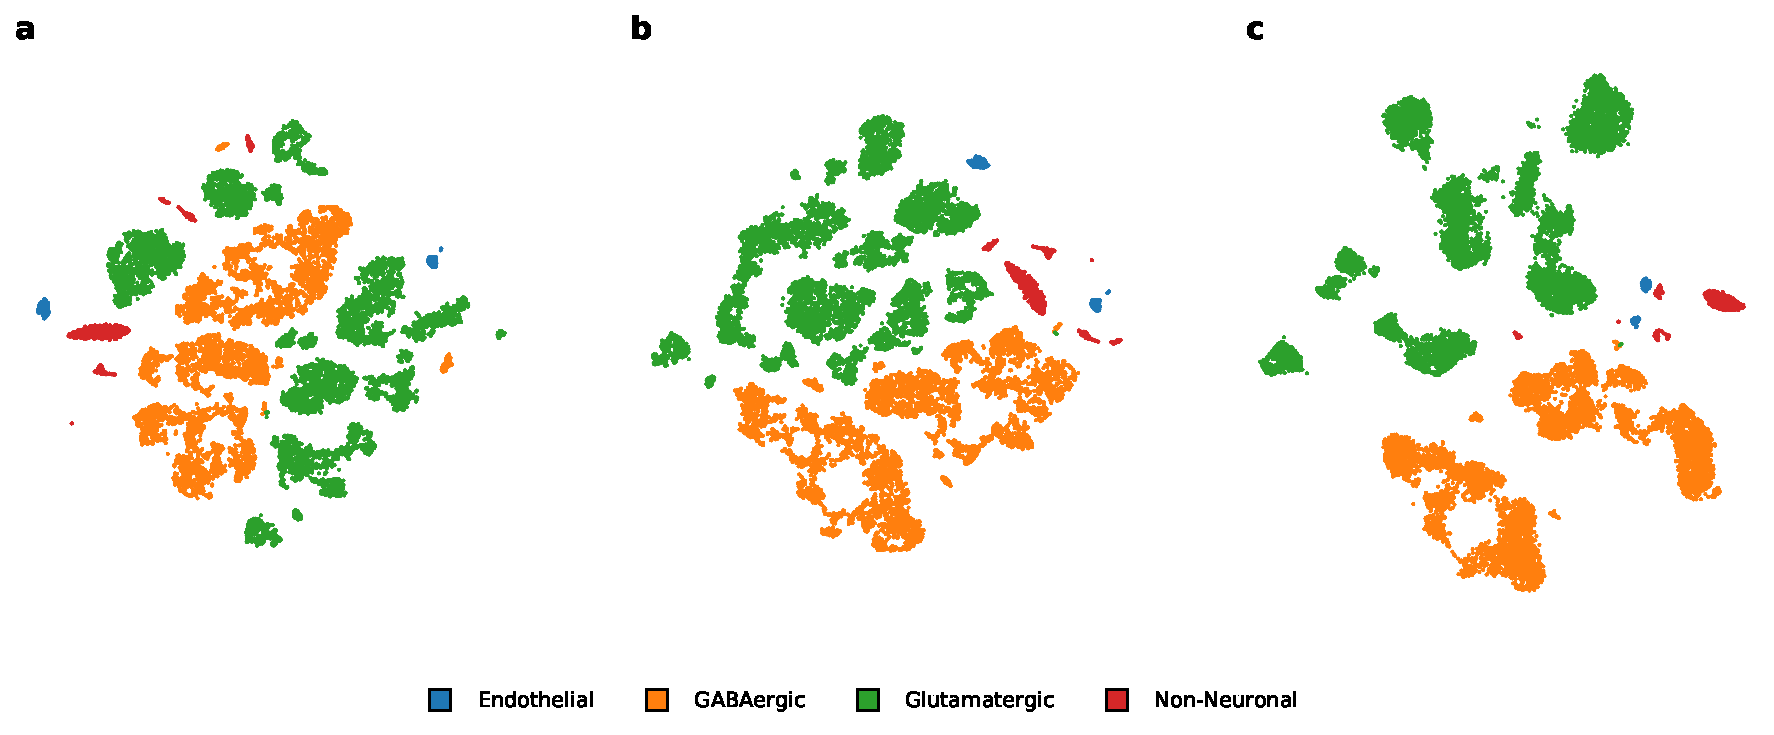
\includegraphics[width=\textwidth]{tasic_multiscale.pdf}
  \caption{A comparison of standard and multi-scale t-SNE on data from the
  mouse neocortex~\DIFdelbeginFL \DIFdelFL{\mbox{%DIFAUXCMD
\cite{tasic2018}}\hspace{0pt}%DIFAUXCMD
}\DIFdelendFL \DIFaddbeginFL \DIFaddFL{\mbox{%DIFAUXCMD
\cite{Tasic2018}}\hspace{0pt}%DIFAUXCMD
}\DIFaddendFL . {\bf (a)} Standard t-SNE using random 
  initialization places clusters arbitrarily. The resulting clustering structure is not globally consistent,
  as clusters of the same type of cells are dispersed throughout the landscape. Non-Neuronal clusters, for instance, are mixed with clusters of GABAergic and Glutamaergic neurons.
  {\bf (b)} By utilizing a globally consistent initialization for t-SNE, the clusters
  are organized in a more meaningful layout, where clusters of cells of the same type appear closer together.
  {\bf (c)} Augmenting t-SNE with multi-scale
  similarities and using proper initialization provides a more meaningful
  layout of the clusters. Non-Neuronal and Endothelial cell types are now placed in
  the same region of the embedding. There are two clear sub-groups of GABAergic
  neurons corresponding to their developmental origins, which was not as apparent
  when using clever initialization alone.}
  \label{fig:multiscale}
\end{figure}

\begin{figure}[htbp]
  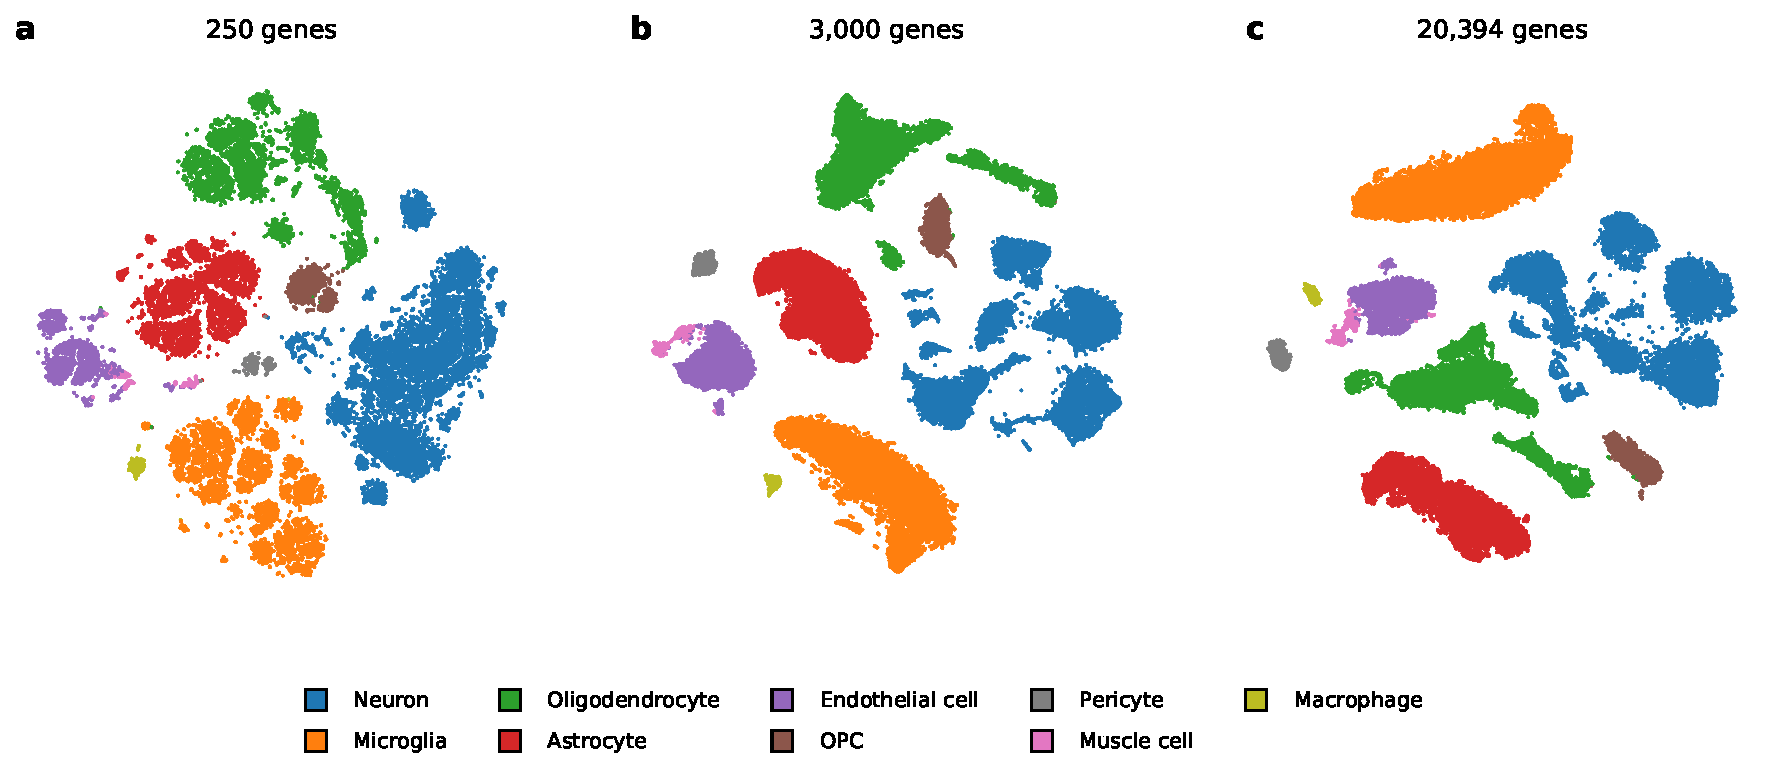
\includegraphics[width=\textwidth]{hrvatin_embedding_tsne_genes.pdf}
  \caption{Gene selection plays an important role when constructing the
  reference embedding. {\bf (a)} Using too few genes results in fragmented
  clusters. {\bf (b)} Using an intermediate number of genes reveals clustering
  mostly consistent with cell annotations. {\bf (c)} Including all the genes
  may lead to under-clustering of the more specialized cell types.}
  \label{fig:gene_selection}
\end{figure}

\end{document}
